\documentclass[12pt,titlepage]{article}
\usepackage{setspace}
\usepackage{fontspec}
\usepackage{pgfgantt}
\usepackage{multicol}
\usepackage{moreverb}
\usepackage{xcolor}
\usepackage{afterpage}
\usepackage{eso-pic}
\usepackage[figuresleft]{rotating}
\usepackage{url}
\usepackage[final]{pdfpages}
\usepackage{graphicx}
\usepackage{caption}
\usepackage{mwe}
\usepackage{subfig}

\def\UrlBreaks{\do\/\do-}
\usepackage
[
        a4paper,
        left=2.5cm,
        right=2.5cm,
        top=2.5cm,
        bottom=2.5cm
]
{geometry}
\setmainfont{Arial}
\pagenumbering{arabic}

\def\signed #1{{\leavevmode\unskip\nobreak\hfil\penalty50\hskip2em
  \hbox{}\nobreak\hfil(#1)%
  \parfillskip=0pt \finalhyphendemerits=0 \endgraf}}

\newsavebox\mybox
\newenvironment{aquote}[1]
  {\savebox\mybox{#1}\begin{quote}}
  {\signed{\usebox\mybox}\end{quote}}

\doublespacing
\usepackage{etoolbox}
\AtBeginEnvironment{quote}{\singlespacing\small}
\apptocmd{\thebibliography}{\raggedright}{}{}

\usepackage{natbib}
\newcommand*{\urlprefix}{Available at: }
\newcommand*{\urldateprefix}{Accessed }
\setcitestyle{notesep={: }}
\bibliographystyle{BCU.bst}

\immediate\write18{texcount -sum -1 \jobname.tex | xargs > \jobname.wc}
\newcommand\wordcount{\input{\jobname.wc}}

\definecolor{bbcnewsred}{RGB}{184,0,0}
\definecolor{bcublue}{RGB}{3,16,51}

\newcommand\NLStart[1]{\AtPageLowerLeft{%
\put(\LenToUnit{.505\paperwidth},\LenToUnit{.12\paperheight}){#1}%
}}%

\newcommand\BCUStart[1]{\AtPageLowerLeft{%
 \put(\LenToUnit{0\paperwidth},\LenToUnit{.12\paperheight}){#1}%
 }}%

\begin{document}

\begin{titlepage}
  \AddToShipoutPictureBG*{
    \BCUStart{\color{bcublue}\rule{.495\paperwidth}{.32\paperheight}}
    \NLStart{\color{bbcnewsred}\rule{.5\paperwidth}{.32\paperheight}}
  }
	\begin{center}
		\vspace*{1cm}

		\begingroup
      \fontsize{24}{30}\selectfont
      \textbf{BBC Feed}
    \endgroup

    \begingroup
      \fontsize{18}{22}\selectfont
      A Novel Interface for News Consumption Inspired by Social Media
    \endgroup

		\vspace{2cm}

		\textbf{Owen Tourlamain}

		\vfill

		Submitted in partial fulfilment of the requirements of Birmingham City University for the degree of Master of Science

		\vspace{0.8cm}

    \begin{multicols}{2}

      \color{white}

  		
\includegraphics[width=0.4\textwidth]{../img/bcu-logo.png}

      CEBE\\
  		Birmingham City University\\
  		United Kingdom\\
      \columnbreak

      
\includegraphics[width=0.4\textwidth]{../img/nl-logo.png}

  		BBC News Labs\\
  		BBC\\
  		United Kingdom\\

    \end{multicols}

    \today - \wordcount words

	\end{center}
\end{titlepage}

\newgeometry{top=2.5cm,bottom=2.5cm,right=2.5cm,left=4cm}

\tableofcontents
\newpage

\section{Abstract}

%To-Do: Write abstract

\section{Research Question}

How could social media user and application interface elements be adapted for
and applied to a digital news consumption platform?

\section{Aims and Objectives}

  \subsection{Project Overview}

  %To-Do: Re-write R and P report

  This project aims to improve upon the application and user interface of
  traditional online news platforms, focusing specifically those used by BBC
  News. The digital news landscape is changing rapidly; a report from Ofcom
  found that people in the UK are increasingly using digital platforms to
  consume news, often through the use of social media \citep{ofcom}. This
  project proposes that adapting user interface and data structure techniques
  from social media and applying them to a news delivery system could increase
  both user engagement and digital journalism efficiency. As the world of online
  news is constantly growing and evolving, the system created will also aim to
  be flexible so that it can adapt to future changes in this space.

  The project will be content-agnostic allowing video, audio and written content
  to co-exist on a single platform. The system will not be limited to those
  three types of media however, it will be designed so that it can work with any
  future media that may be devised. To achieve this, the project will be divided
  into three parts: the feed, the catalogue and the scrapers. The feed will be
  an app that users can interact with. It will need to intelligently select
  content from the catalogue and present it to the user for consumption. The
  catalogue will store content that can be displayed, this will aim to be fast
  to access, and well organised to ensure a smooth flow of content to the users.
  The scrapers will create the content for the catalogue by connecting to
  various BBC news data sources. They will read this content, translate it into
  a form suitable for the catalogue and store it. Creating these scrapers will
  involve writing specific interfaces to many different sources of news content;
  as this will take a lot of time they will not be produced as part of this
  project however they will be considered when developing the API for the
  catalogue portion.

  Social media often faces criticism for being addictive and of wasting users
  time \citep{neyman}. This raises ethical considerations with this project as
  it has the potential to also create these same issues. This will be mediated
  by the lack of user created content, meaning that the users time will be spent
  browsing informative news rather than wasting it. The addictive nature of
  social media is actually a benefit to this project as it is trying to increase
  user engagement on news platforms. As this project is focusing on the
  interface implementation the user experience is out of scope here, and will
  not be measured in any way. This is an area that a future study may wish to
  explore however as the ethical considerations around increasing user engagement
  time are both interesting and important to understand.

  \subsection{Key Terminology}

  \textbf{Infinite scrolling}: A user interface paradigm that presents content in a
  scrolling window. Before the end of the content is reached more content is
  loaded, resulting in the content appearing infinite to the user. This is often
  seen in social media, for example Facebook's news feed, and Twitter's timeline.

  \textbf{News Content}: For the purposes of this study news content will be
  defined as text, audio, images or videos that are created or distributed by a
  news agency. These can come from a variety of sources ranging from broadcast
  news programmes to stock photos used within an article.

  \subsection{Deliverables and Goals}

  The deliverables for this project will be two of the three components
  highlighted above, as well as all documentation required to understand,
  maintain, deploy and use the system. The documentation will be provided in a
  plain text readme file formatted using markdown, this has been chosen because
  the format works well with GitHub which will be used throughout the project.
  This documentation will be supplemented with comments within the code base. The
  majority code produced will be written in Python, with HTML, CSS and
  JavaScript used for the web interface. Also included will be a set of test
  data that can be used to demonstrate the system in a working state.

    \subsubsection{The Feed}

    This deliverable will use Python's Flask module, a light-weight web
    application framework that has been chosen due to its simplicity and lack of
    overhead. The python application created will be able to either be run
    locally or deployed to a web server. It will have accompanying scripts that
    install any prerequisites for running the application. This deliverable will
    depend on having a valid catalogue to read from.

    \subsubsection{The Catalogue}

    This will consist of a Python module that will provide an interface to a
    database holding test data. In a production environment this database would
    be hosted on a saleable cloud system, such as AWS RDS. For this project
    however, a local SQLite database will be used.

    \subsubsection{Test Data}

    This will take the form of a single file containing SQL data that can be
    loaded by the catalogue to initialise its database with test data. The
    contents of this data will be sourced from the BBC News website.

  \subsection{Out of Scope Issues}

  This project is primarily focused on the engineering challenges of developing
  this system, as such it will not be attempting to measure user experiences in
  any way. The project will also not be attempting to judge the performance of
  any content selection algorithms that are used. These topics are highly
  important to the problem space being explored, however they each could
  constitute a project in their own right and would spread the focus of this
  project too thin. These two issues would make for excellent follow up projects
  however so some comments may be made where relevant to future research.

\section{Background and Rationale}

  \subsection{Overview of the Problem Space}

  Modern news consumption started with the newspaper. Despite moving to online
  platforms these roots can still be seen in the user interfaces of digital news
  platforms such as the BBC News website and mobile app \citep{ofcom}. These
  interfaces broadly function by providing categories of content to browse, this
  makes these interfaces good for researching topics and for getting an overview
  of recent news within a topic \citep{yalanska_2021}. Social media instead often
  delivers content to users through an infinitely scrolling feed. This style of
  interface fits well with short bursts of interaction, such as while waiting
  for a kettle to boil or waiting for a bus \citep{yalanska_2020}. In these
  scenarios users often want to consume content without having to choose a
  category or risk running out of content.

  This style of interface removes the need for the end user to decide what
  content they consume at the point of consumption, instead they control what
  content is presented to them by following, liking, subscribing to or otherwise
  choosing to receive content from a number of sources. From this user input a
  social media platform will choose exactly which content to provide to a user,
  and in which order. The specifics of how these decisions are made are closely
  guarded secrets, and as such will not be investigated here.

  While social media allows users to access news content in this way, it is
  often preferential to deliver news to users on a first party platform, such as
  the app or website of the news agency. This gives the producers of the content
  more control over how it is presented and consumed, as well as what other
  content may be presented to the user alongside the current content. This
  project aims to create an interface inspired by social media, but completely
  controlled by the news agency.

  This also gives the creators of this content more flexibility to experiment
  with new content types, they are not limited to the narrow selection of media
  that the various social platforms offer. This feed can also offer features
  such as A/B testing that would enable the content producers to test the
  effectiveness of new media types \citep{ab}.

  When creating printed media, such as a newspaper, each article or photograph
  that is included takes up space that could have been used for something else.
  Because of this it is key to only select content that will have the greatest
  impact, and testing new content is risky. In an infinite scrolling style of
  interface however there is no limit on the amount of content that can be shown
  to a user, as such inserting new media forms to test them becomes more viable
  as if the user is not interested they can scroll past and move on to the next
  piece of content.

  \subsection{Motivation for the Project}

  The BBC runs a news innovation team, called News Labs, which develops novel
  technologies for news creation, consumption and delivery. Two of their recent
  projects, which formed the inspiration for this project, are SlicerAV and Live
  Segment Notifications (LSN) projects. SlicerAV takes broadcast TV and radio
  news programmes and automatically breaks them up into 'slices' of short form
  media \citep{slicer}. Once this project was functional the next question was
  how to deliver this content to end users. For testing purposes they decided to
  tweet the slices as it was identified that the content fit well on to a social
  media platform, and twitter worked best for this use-case.

  The LSN project aimed to inspect news broadcasts just before they go live and
  notify users about upcoming content, in the form of 'slices', that may be
  interesting to them \citep{lsn}. This was successful, however it did not fit
  well with the current BBC online news delivery systems. This raised the
  possibility of a feed that would hold all the slices that a user had been
  notified about for them to browse. This idea was considered and built upon,
  eventually leading to the idea of a unified news homepage, where sliced
  content could be surfaced alongside regular articles and videos.

  News Labs is focused on innovating news creation, consumption and delivery, as
  such they have several projects that could benefit from a flexible user
  interface to surface their content. One such project is Graphical Story
  Telling (GST) which aims to take articles and turn them into a series of
  graphics with overlaid text that can be swiped through \citep{gst}. This
  content is inspired by social media and would fit perfectly into this project.
  This provided the idea to make a flexible feed that can present a wide variety
  of content in one place, with functionality for personalisation and testing.

\section{Literature Review}

  \subsection{Interfaces for Online News Consumption}

  Since the popularity of online news has taken off, there has been a lot of
  innovation and experimentation into the interfaces we use to consume this
  media. Most news agencies have tried to move away from simply displaying walls
  of text to users, in the work of \cite{msnbc} we see a case study into how one
  large news agency re-designed their user interface, and the software stack
  that runs it. This study highlights how important flexibility was in the
  system. They split the system between the front end and the back end with the
  goal that "User interfaces and databases would become isolated components to
  be updated and swapped out" \citep{msnbc}. This closely mirrors the model
  proposed in this project. The case study also made note of the new system
  allowing content to reach audiences that hadn't been considered targets when
  the content was produced:

  \begin{quote}
    The same trading zone-style compromise also made it possible to take advantage
    of moments of alignment between editorial staffs and products whose tenor and
    target audiences might be viewed as incompatible on a larger scale.
  \end{quote}

  This shows that the connections to the SlicerAV project should prove useful,
  as that will allow segments of broadcast programmes to reach audiences that
  the whole programme may not.

  Some projects have taken this redesign in a different direction, in the work of
  \cite{newsstand} we see an attempt to display news content based on it's
  geographical location. Localised news has always been popular, with the BBC
  running separate news programmes for different UK regions. This approach would
  allow a user to browse content purely by location which may have advantages to
  both end users and content producers. A map interface will not be a part of
  this project, however it is worth keeping in mind when building the data
  structures so that out of the box ideas like this can be built in the future.

  One key element to all major user interface redesigns is that they should be
  an improvement in some regard to the old system. Whether that is measured in
  loading speed, running costs, or any other metric, the improvement should be
  measurable in someway. Testing the proposed system against the current BBC
  News user interface would be a monumental task, requiring data that cannot be
  easily accessed. As such the measurement is out of scope for this project,
  however the means to perform those tests should be built into the system. In
  order to identify which metrics are important to track we can look at the
  published work of \cite{ux} and \cite{engagement}. \cite{ux} highlight that
  simple metrics, such as time spent browsing or number of articles viewed, are
  not sufficient on their own as both high and low figures for these can
  indicate good and bad user experiences. The authors also found that the best
  way to measure user engagement was through interviews, this would be
  impractical to use all the time. Instead this project will aim to include some
  form of user feedback into the system, this will likely be modelled on a
  favourites system or a positive/negative indicator.

  \subsection{Infinite Scrolling User Interfaces}

  \citep{newtarget} defines infinite scrolling as:

  \begin{quote}
    a technique that allows users to scroll through a massive chunk of content
    with no finish line in sight. This technique simply keeps refreshing a page
    when you scroll down it.
  \end{quote}

  This description highlights how simple this design pattern is from a users
  point of view, but goes on to show how much of an impact it can have on the
  users. It states that users often feel that they "might be missing out on
  information" \cite{newtarget} as there is always more content being added to
  their screen. One possible solution it offers for this is some form of marker
  to show users how far they have gotten in the list and allow them to return
  later, this will be considered as a feature for this project.

  \cite{neyman} and \cite{karlsson} have looked into the negatives of infinite
  scrolling interfaces, highlighting the addictive nature and that users often
  waste time while using them. For the purposes of this project however these
  features are actually helpful as there is a desire to increase engagement on
  the BBC News platforms, and the users time will not be wasted as they will be
  browsing informative and well written news articles. Both studies do however
  note that too much choice can be a bad thing, \cite{karlsson} state:

  \begin{quote}
    while people may be attracted by a large variety of options, they are more
    likely to act when given fewer choices.
  \end{quote}

  This is something to keep in mind when designing this system, the project
  should aim to not overload the user with too many options at once. Techniques
  such as allowing users to save articles for later, return to their position in
  the list and allowing them to filter content to different categories will help
  to overcome this.

  Another aspect to consider is the implementation, as mentioned by
  \cite{newtarget} infinite scrolling has the potential to reduce the
  responsiveness of the interface as more content is loaded. \cite{tajima} used
  SuperSQL in order to work around some of these issues, this may be a fitting
  technique for this project as it will be using a relational database. As a lot
  of content will have to be loaded, small delays between system components will
  quickly add up resulting in a poor user experience. To combat this each
  element of the system will need to be tested thoroughly and UI tasks such as
  rendering should be separated from other logic through threading.

  \subsection{Social Media Design for Increasing User Engagement}

  Social media is not a new concept to news distribution. \cite{standley} found
  in a survey that social media is now the most commonly used communication
  channel on the internet. \cite{boukes} found that social media ranked highly
  as an important source for news, especially among younger audiences. This has
  naturally caused many news outlets to start publishing content on social
  media, this however has not come without any downsides. \cite{boukes} showed
  that "Twitter usage positively influenced knowledge acquisition [and] Facebook
  had a negative effect", they suggest that this is co-related to the target
  users of the platforms, stating that twitter users are often motivated to use
  the platform to gain knowledge and information. This means that using these
  techniques on a news app or website should work well, as the audience will have
  visited the service with the purpose of gaining information.

  This project has one key difference from social media, in that it will not
  contain any user made content. \cite{zhang} found that an infinite feed
  increased appreciation of content produced by others, but decreased users
  desire to create their own content. Since there will be no ability to create
  user content this will not be an issue for this project.

  There are a lot of negative effects often associated with social media. As
  this project is taking inspiration from this area it is worth taking steps to
  ensure that these negatives are not a part of this new system.
  \cite{lupinacci} suggests that a lot of these issues stem from a state of
  "continuous connectedness" to other people. Users will not be connected to
  each other in this system, however they may still experience these issues by
  being constantly connected to the world through the news. The best way to
  avoid this is a topic for a study in it's own right, for this project it is
  sufficient to be aware of the issue if it appears.

\section{Methodology and Planning}

  \subsection{Development Methodology}

  The development of this project will follow a Kanban-style methodology
  \citep{kanban}. Since there is only one developer on this project this will not
  be used for collaborative purposes, instead it will be used to manage and
  monitor tasks. As tasks arise they will be added to a To-Do list. These will
  me moved to an In Progress list when they are started and then a Done list
  when finished. Tasks will be added, edited and split into sub-tasks as needed
  throughout the project. This methodology will allow a high degree of
  flexibility which fits the project well as the specifics of the project will
  likely evolve as the project progresses.

  Test driven development was considered for this project. It would help to
  increase system reliability and enable the testing of the system to be
  efficiently tracked and repeated when necessary. These features however aren't
  key to this project as the focus is around prototyping and rapid development.
  Using a methodology such as test driven development would add more overhead to
  the project and slow down progress. The risk of reducing the robustness of the
  system has little impact as this project will never be deployed in a live
  setting.

  \subsection{Project Timeline}

  Time management for this project will be monitored through the use of a Gantt
  chart (see fig. \ref{fig:gantt}). Contingency time takes the form of two week
  long blocks where no development is planned. Depending on how the development
  progresses this time will either be used for further research and writing, or
  more development time. This chart will be updated as the project develops and
  objectives are added or removed, however individual daily tasks will not be
  added. These will be tracked through the Kanban board mentioned later in the
  methodology.

  \clearpage

  \begin{sidewaysfigure}
    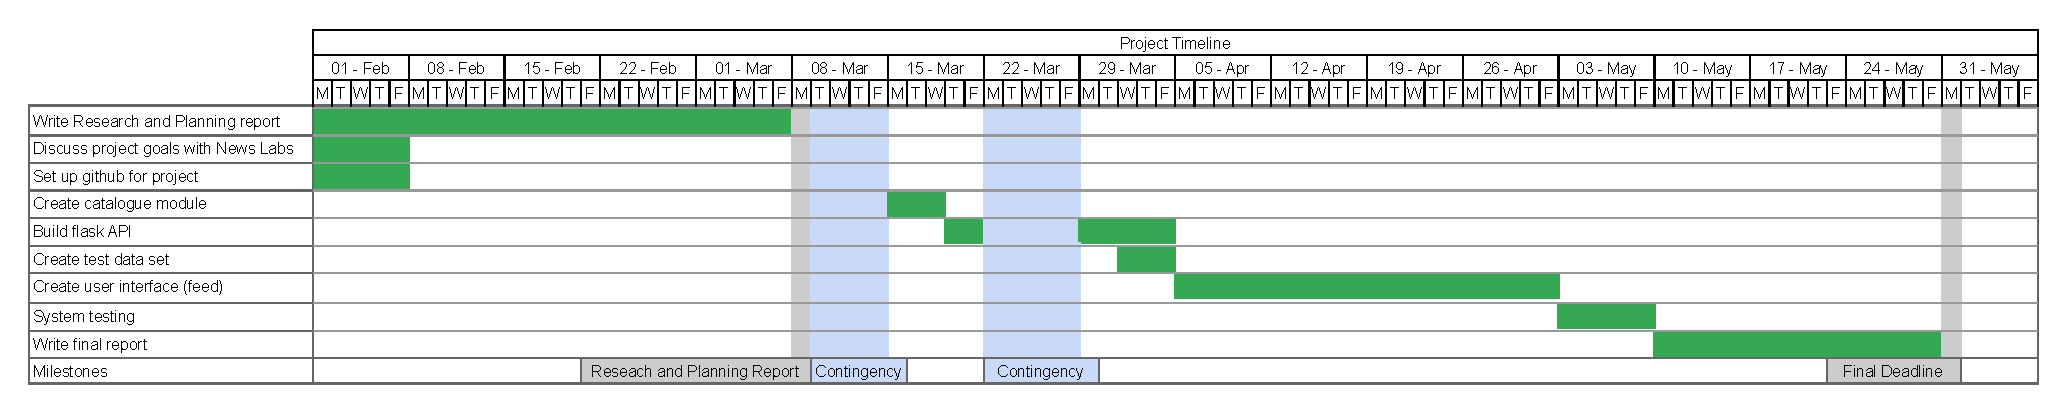
\includegraphics[width=\textheight]{../img/gantt.pdf}
    \caption{Project timeline gantt chart}
    \label{fig:gantt}
  \end{sidewaysfigure}

  \clearpage

\section{System Development}

  \subsection{Development Methodology}

  Throughout this project an iterative development style was used. This took the
  form of a 'design-implement-test' loop that was repeated for each step of the
  project. Tasks were taken from the Kanban board, implemented and tested before
  moving on to the next task. This was used to provide compartmentalisation to
  the system; each element performs a simple function that could be tested
  easily. When each of these elements are connected they create a more complex
  system.

  A good example of this is the API side of the catalogue module. This uses SQL
  commands to retrieve information from the database and convert this
  information into Python objects. As part of this it is necessary to link some
  objects together, every \textit{post} belongs to a \textit{story} for example.
  Rather than writing specialised code to create this link each time, the
  existing \textit{get\_story()} method was used.

  This compartmentalisation also streamlined development significantly as each
  element could be re-written independently of the rest of the system. This
  flexibility was utilised heavily when the catalogue module had to be
  re-written to support large changes to the database structure. It was simple
  to change the code within the module without affecting the rest of the system.

  Using test driven development was considered for this project; it would have
  provided structure and repeatability to the testing procedure. However this
  would also have added significant overhead to the development of the project.
  As the project was heavily time restricted, and the output was focused around
  the user interface rather than the technical implementation, it was decided to
  use a methodology with less process overhead.

  \subsection{Language and Technology Choices}

  Language and technology decisions for this project were guided by the need for
  rapid development and the prototype nature of the system. As long term
  maintainability and reliability were not priorities for this project, the
  focus was instead on choosing technologies and languages that would facilitate
  rapid development and innovation. As such, the chosen platforms are all ones
  that the author has a lot of experience with.

  The core of the project was implemented in Python 3.7, this was chosen as it
  is a recent version of Python that runs well on the hardware used for
  developing the system. To create the API and back-end portions of the system
  Flask was used as this fit well with the rapid prototyping nature of the
  project. Flask also provides the Jinja template rendering engine which made
  producing web pages fast and efficient. These pages were built using pure
  HTML, CSS and JavaScript as this avoided having to learn new user interface
  frameworks.

  \subsection{Development Progress}

  The first section that was implemented was the initial catalogue and API.
  These needed to be developed concurrently as they are very tightly coupled. It
  would also have been difficult to test the catalogue without the API present,
  and vice versa. The structure for developing these elements was to select a
  table from the database and implement it in catalogue with \textit{add} and
  both singular and multi-item \textit{get} methods, these were accompanied by
  matching API endpoints.

  Once all of the tables were represented in this fashion, work was started on
  the user interface. To develop this, static web pages were first written.
  These had no connection to the data stored in the catalogue and were used to
  develop the interface without worrying about the data interface working
  correctly. Once a page was finalised the static elements were replaced by data
  read from the catalogue. The use of Jinja as a template rendering engine made
  this step simple and greatly streamlined this area of development.

  At this point a basic web interface had been developed and the next step was
  to add functionality to the site. Each feature was roughly prioritised based
  on time to implement and benefit to the system. Adding a functional log in
  system was quite time consuming, however it was vital for other elements of
  the system to function at all so this was given a high priority. As part of
  this process several new methods needed to be written in order to support new
  features. For example, it was required that users could be retrieved by name
  rather than by ID for the log in system to function correctly.

  \subsection{Issues Faced}

  The main issues faced during the project were around the need to balance the
  benefit of adding a feature with the time it would take to implement. The best
  example of this is when it was realised that a ground up re-write of the
  catalogue module would be highly beneficial to the project, however it would
  also take several days of development time. It was decided instead to find a
  work around that would take much less time to develop. This method of task
  prioritisation was vital to ensure the project was completed within the
  time frame required.

  The time constraints of the project also required that some desired features
  be cut from the system. It was decided early on in the project timeline to
  remove the data gathering portions of the system. This allowed the project to
  become more focused around the user interface implementation, as creating
  placeholder data was significantly faster.

\section{Final System Overview}

  The final system consists of two main components that provide the
  functionality and user interface of the system respectively which are detailed
  below. In addition to these components there is a database schema and
  prototype data set which have been produced.

  \subsection{Catalogue}

  The catalogue portion of the system has been built as an independent Python
  module, the aim of this was to encourage de-coupling the data model
  implementation from the rest of the system. This allows the data source to be
  swapped out very easily and would allow the use of saleable cloud-based
  databases such as AWS RDS.

  The main functionality of the module is provided by \textit{catalogue.py}, as
  shown in fig. \ref{fig:catalogue}. In this file is a single class, called database,
  that handles all the interaction with the SQL database. When this class is
  initialised it attempts to access a database file, creating it if the file
  doesn't exist. If the database is empty it initialises it with a pre-written
  database schema and test data. This was done to reduce the development time
  needed to maintain the database as it could be quickly wiped and rebuilt with
  minimal effort.

  \begin{figure}
    \centering
    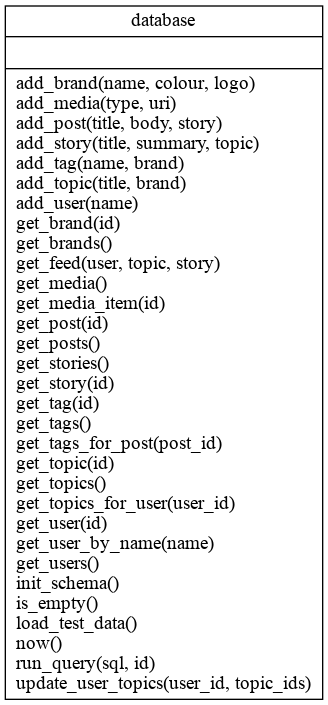
\includegraphics[height=\textheight/3]{../img/catalogue.png}
    \caption{Database Class}
    \label{fig:catalogue}
  \end{figure}

  All database tables have an \textit{add} method, as well as \textit{get}
  methods for both single items or all items in the table. In a full production
  system it would be necessary for this module to provide \textit{create},
  \textit{read}, \textit{update} and \textit{delete} methods for all data. It
  was decided that this would take a long time to develop and would add minimal
  functionality to the project so the update and delete methods were not
  implemented. In the final system the \textit{add} methods were hardly used due
  to the data scraping part of the project being removed, however implementing
  these methods has provided an API for automated data entry.

  Some of the \textit{get} methods have to link multiple items together, for
  example every \textit{post} belongs to a \textit{story}. This was achieved by
  having the relevant methods call other methods from the same class, for
  example \textit{get\_post} calls \textit{get\_story} using the \textit{story\_id}
  from the post. This method in turn calls \textit{get\_topic} which calls
  \textit{get\_brand} to complete the post item. With a longer development
  time frame a better solution to this problem could have been found by utilising
  a pre-written Python object relational mapper such as SQLAlchemy. This would
  have made the data management side of the project much simpler, however it
  would have also imposed limits on which data technologies could be used which
  would have reduced the independence between the database and data management
  system.

  The rest of the methods in the class provide specific data access as needed by
  other elements of the system. Methods such as \textit{get\_user\_by\_name} are
  required to fulfil a specific purpose and were added as and when the need
  arose during the project development. For example \textit{get\_user\_by\_name}
  was added to improve efficiency when checking if a user exists in the
  database. Only one update method was required during the project, this was to
  allow users to change their topic preferences through the web user interface.

  \begin{figure}
    \centering
    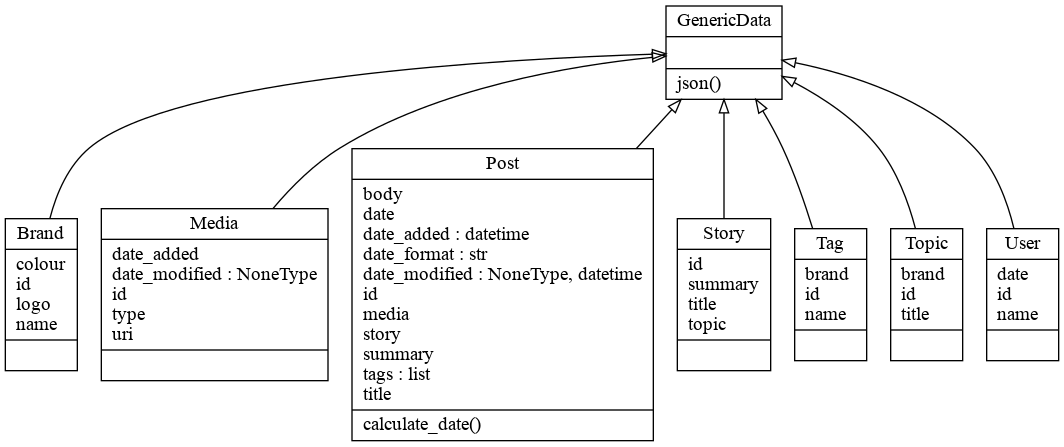
\includegraphics[width=\textwidth]{../img/datatypes.png}
    \caption{Datatypes Classes}
    \label{fig:datatypes}
  \end{figure}

  The second file in the module, \textit{datatypes.py} as seen in fig.
  \ref{fig:datatypes}, provides a collection of classes that represent the
  various datatypes stored in the database. This was created to allow the other
  parts of the system to interact with the data in a Pythonic, object-oriented
  way. By using this interface the other parts of the system don't need to worry
  about the specifics of the database schema or engine. Each of the datatypes
  inherits from a base class called \textit{GenericData}, this provides shared
  methods which allow the datatypes to be compared and also serialised into a
  JSON format for the REST API.

  As it stands the project implements zero authentication or security to any of
  the endpoints or database. Currently if the project was hosted online anyone
  who knew the endpoints could inject data into the catalogue easily, and anyone
  with access to the host machine could connect directly to the database to
  manipulate the data. In a production environment these issues would need to be
  addressed. The API would implement authentication where allowed applications
  could receive a token that would allow them to access the API endpoints.
  Additionally security certificates could be used to ensure that requests are
  originating from valid systems. The database wold also have to be secured by
  creating users with limited permissions and passwords, in addition to this the
  host machine would need to be secure to ensure attackers cannot access the
  system this way. These issues were not resolved in this project as it will
  never be hosted or used in a production environment, however they would need
  to be addressed if the project was developed any further.

  \subsection{Feed}

  The feed portion of the system provides a web based user interface as well as
  a RESTful API, using Flask to process these requests. Both of these are
  contained in \textit{app.py}, using different endpoints to differentiate the
  two interfaces. The endpoint structure has been designed so that all the API
  endpoints end in \textit{/json/}; this means that for most user interface
  pages \textit{/json/} can be appended to the URL to retrieve the data in JSON
  format.

  The API side of the Flask app provides an endpoint for each of the basic add
  and get methods that the catalogue supports. These endpoints can be used to
  add data to the system from external sources. As these external services would
  not need to modify or remove data so these endpoints were not added.

  The rest of the endpoints provide the various user interface pages. Each is
  written as a Jinja template using plain HTML, CSS and JavaScript. The
  templates were designed to be modular wherever possible, this allows common UI
  elements such as the navigation pane to be reused between pages. The UI design
  follows BBC guidelines wherever possible, Including making use of the BBC font
  Reith Sans, and using a header and footer designed by BBC News Labs. These
  elements were included to help the UI feel more authentic, which makes the
  final system easier to compare to current news platforms such as the BBC News
  website. This was reinforced by the use of the official BBC UI and branding
  colours.

  The novel elements of the UI were inspired by social media feeds such as
  Facebook's news feed and Twitter's timeline. This lead to the vertically
  scrolling list of posts, which allows users to easily consume news articles or
  scroll past them if they are not interested. One interesting UI development
  was the expanding posts, this allows for users to consume more content they
  are interested in without interrupting their scrolling. This keeps the UI
  focused on a single page experience, rather than directing users to multiple
  pages which could lead to navigational issues.

  The feed implements very basic authentication, however this is only based on
  the user name and no password or other form of secret is used to secure these
  accounts. In a production environment this would cause major issues, however
  implementing these features would have added significant development time
  without contributing to the user interface or other features of the project.
  As this project is only a prototype and will not be deployed anywhere it was
  decided that not implementing this was acceptable

  \subsection{Database}

  \begin{figure}
    \centering
    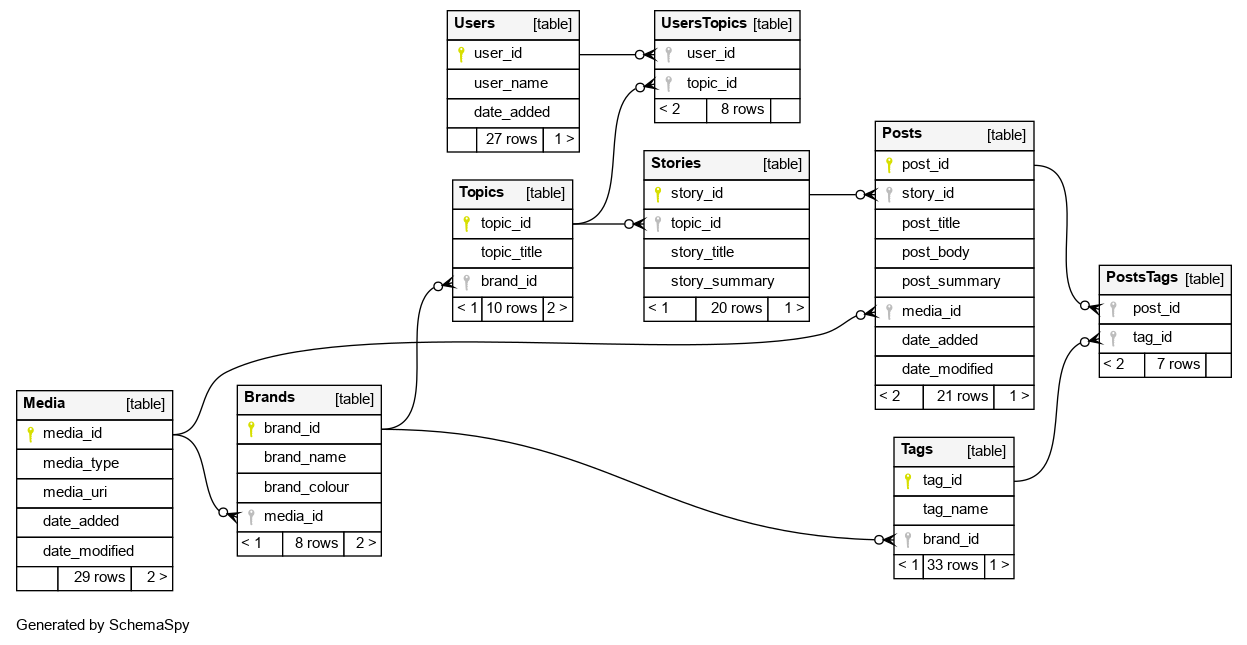
\includegraphics[width=\textwidth]{../img/dbschema.png}
    \caption{Datatypes Schema}
    \label{fig:schema}
  \end{figure}

  The database has been designed to show how the use of intelligently structured
  data can effect the delivery of online news. The core data structure in the
  system is the relation between \textit{posts}, \textit{stories} and
  \textit{topics}. Using this structure posts can be collected under their
  stories, which in turn can be grouped and filtered by topic. This allows for
  user interfaces to display content in a form which reflects the dynamic way
  that news stories develop and grow. This structure allows data to be inserted
  into the system from many sources all contributing to the same set of stories.

  To achieve this structure the database had to be built to be designed
  following industrial best practices. As such it was normalised to the third
  normal form, this ensures that the data is stored logically and to eliminate
  redundant data. The best way to achieve this was to make sure that each record
  in the database was atomic, meaning that it only contains one item. For
  example each \textit{user} can have multiple \textit{topics} that they are
  following. To represent this 'one-to-many' relationship in the database an
  extra table was created that holds pairs of \textit{(user\_id, topic\_id)}
  that can easily be queried to extract the followed topics for a given user.

  To make the database easier to maintain the schema has been defined in a
  separate file that can be loaded on start up, this schema can be seen in fig.
  \ref{fig:schema}. This allows the structure of the database to be changed with
  minimal effort, and even swapped out for a completely different one if
  desired. In a similar manner the test data is stored in plain text as a
  sequence of SQL \textit{INSERT} commands, Keeping these two files in plain
  text allows them to be version controlled along with the rest of the system,
  this helps streamline development and track changes throughout the process.

  \subsection{Changed and Removed Features}

  Due to the time constraints on this project paired with its ambitious nature,
  several features had to be simplified or cut entirely. Deciding which
  features to remove or change required analysing each one and weighing the
  benefit it would bring to the project, against the time and effort it would
  take to implement. Some removed features required other simpler systems to be
  built to replace them; the time and effort cost of these were considered
  as well.

  The largest of these cut features was the external data gathering programs.
  These would have collected data from various BBC sources and fed this into the
  catalogue. This feature would have highlighted the way this system allows for
  disparate data from a variety of sources to tell a coherent story.
  Implementing this would have taken a large proportion of the development time
  available to the project as finding appropriate data sources would have
  required contacting many different teams within the BBC in order to work out
  how the data could be ingested. Coordination across an organisation as large
  as the BBC typically spans weeks, if not months, which would not work within
  the time frame of this project. Once these data sources were identified
  bespoke software would need to be written for each one and hosting solutions
  would need to be found to ensure that they could gather data effectively. This
  feature was emulated by creating a set of test data that represents how the
  system might appear if these data gatherers were operational. This emulation
  is sufficient to prove the concept of the the system so making this
  replacement was deemed beneficial to the project

  One key aspect of social media is the ability to interact with content through
  a feedback system such as using 'likes' or 'dislikes'. The initial conception
  of this project included a similar system that users could use to indicate
  content they were interested in or content that they did not want to see more
  of. The feed would then have shown the user more or less of a specific topic
  depending on their interests. One issue with this idea is it requires the
  system to make choices on behalf of the user, how many times should a user
  dislike a topic before it is removed from their feed? Developing a system that
  can make these choices, and tuning it to give the desired outcome is a
  significant task that would constitute a research project all of its own. As
  such it was decided instead to simply let the user pick which topics they are
  or are not interested in via their user profile. This method allows the rest
  of the project to demonstrate how such a recommendation system would affect
  the user interface without needing to dedicate the time to developing such a
  system.

  As the current BBC News website offers both a desktop and mobile experience,
  it was initially desired to create both of these for this project. It was
  decided however that splitting development effort between two separate
  interfaces would have negatively impacted the project and as such the mobile
  interface was not implemented. The option to have different interfaces for
  different use-cases was considered when developing the project. This lead to
  the choice to use a template rendering engine as this allows for a different
  template to be rendered depending on various factors, such as if the user is
  accessing the site through a mobile device.

  \subsection{User Interface}

    \subsubsection{Home Page}

    \begin{figure}

      \begin{minipage}{.5\linewidth}
        \centering
        \subfloat[Default view]{\label{fig:home1}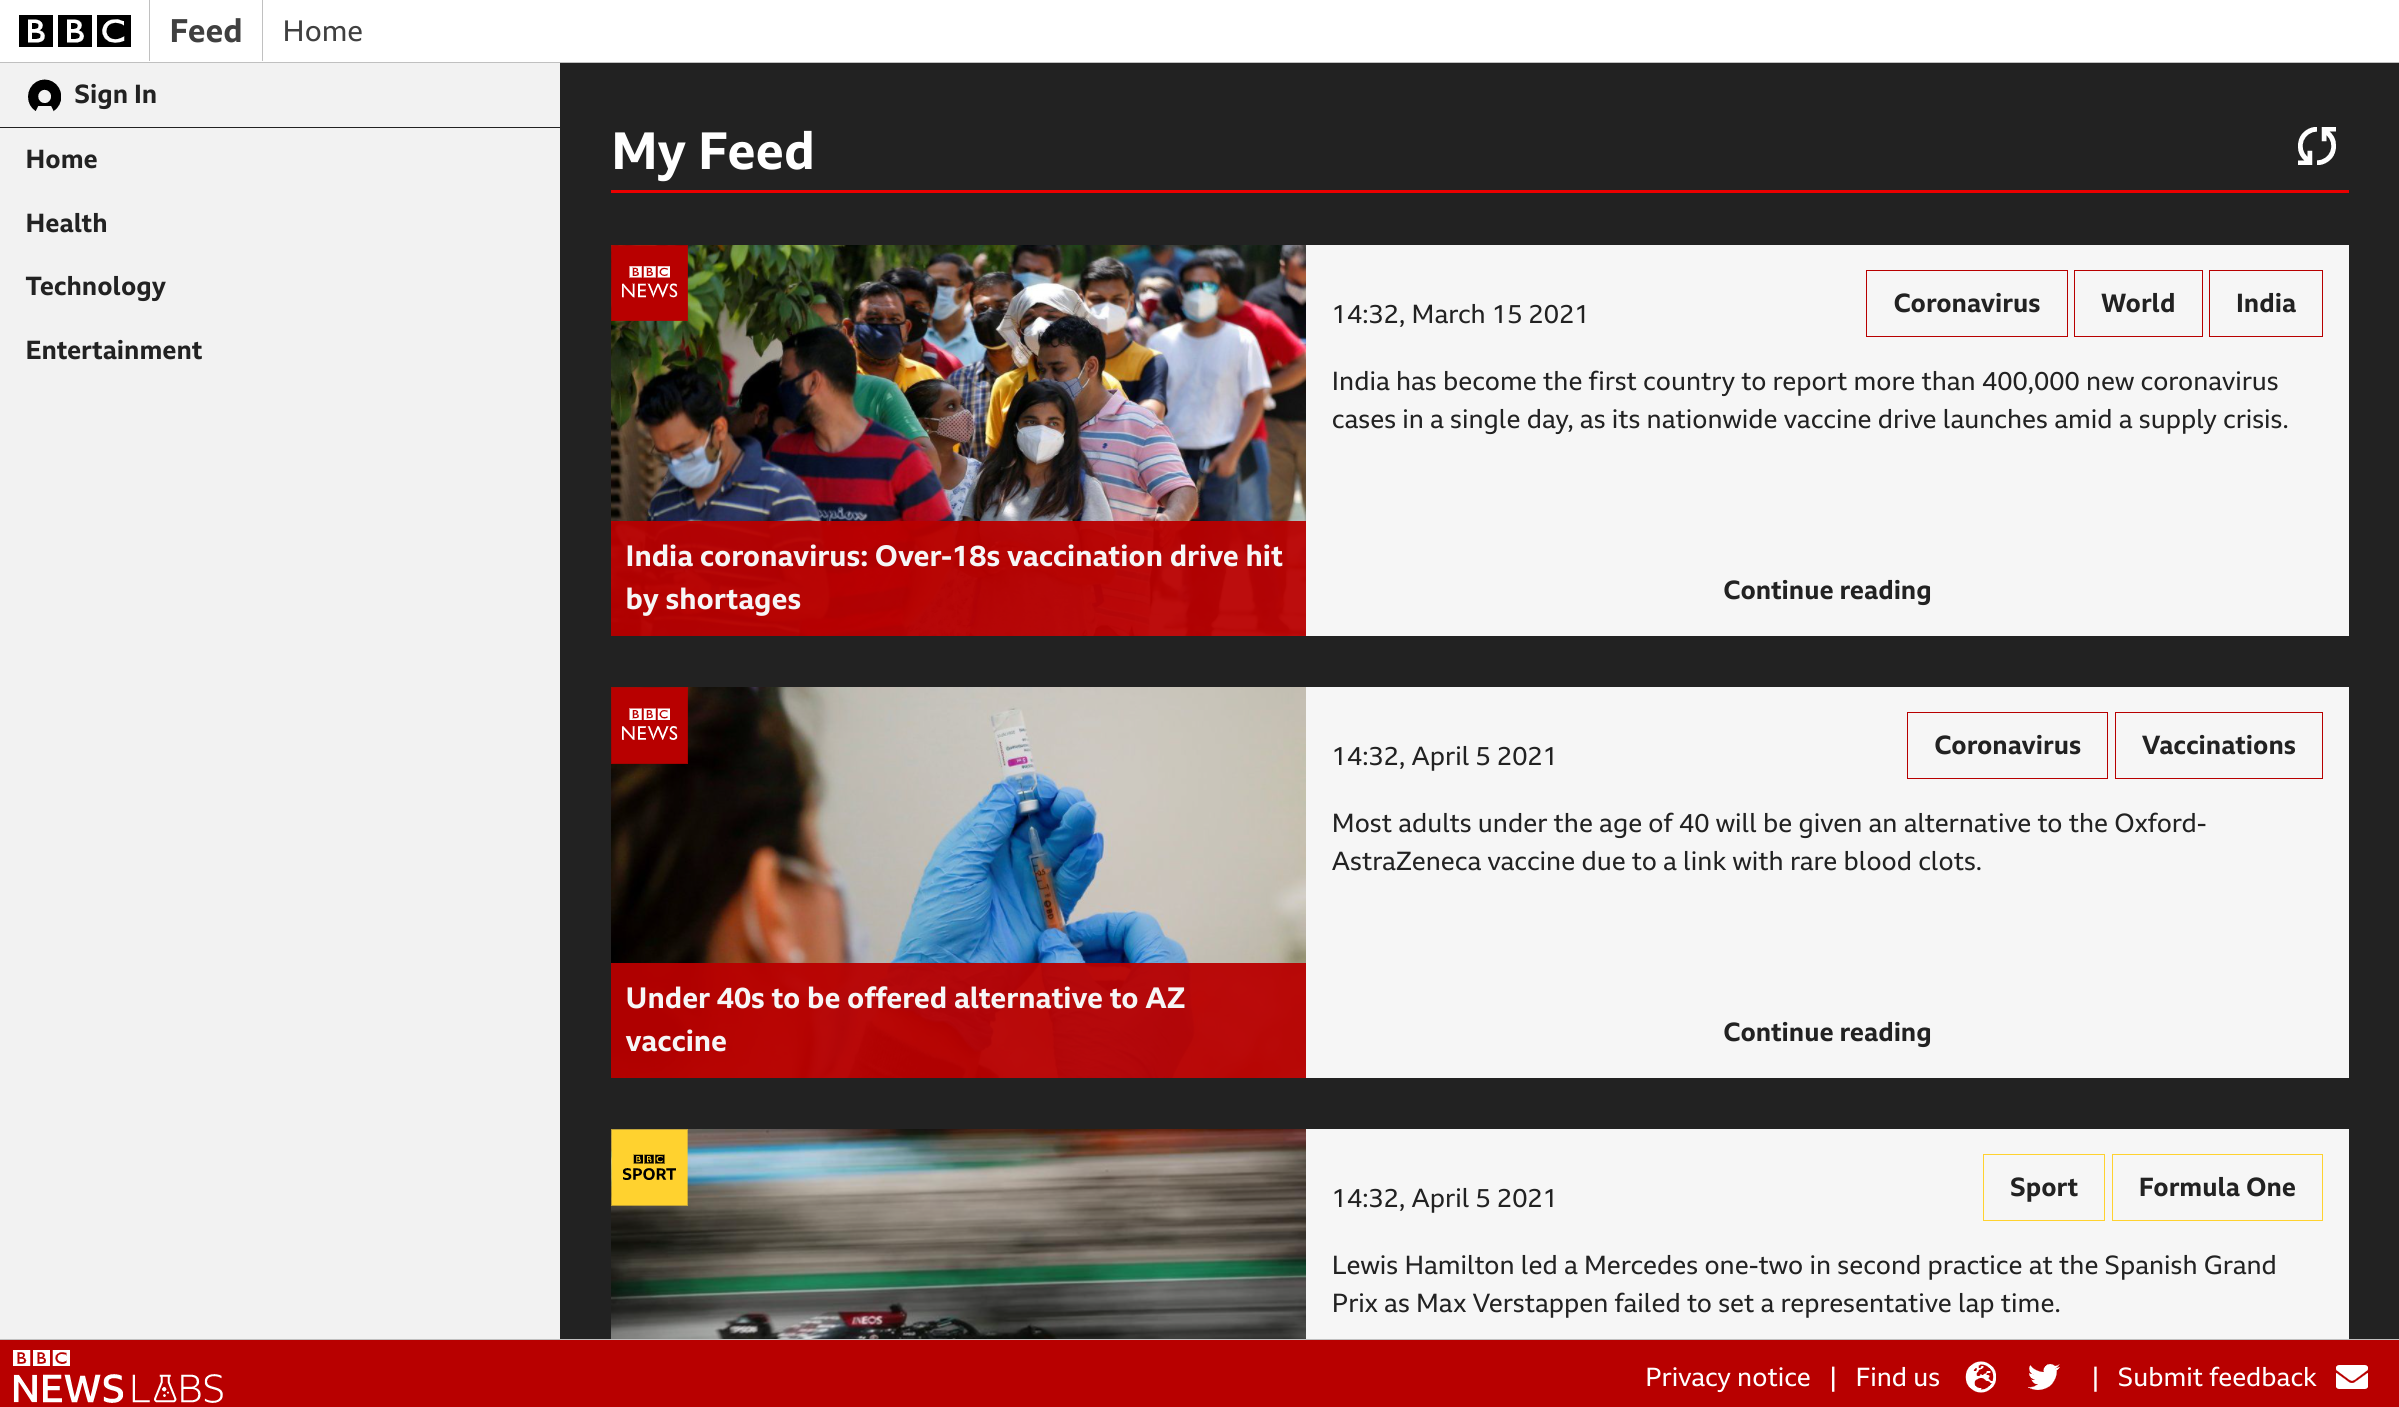
\includegraphics[width=.95\linewidth]{../img/sc-home.png}}
      \end{minipage}%
      \begin{minipage}{.5\linewidth}
        \centering
        \subfloat[Signed in]{\label{fig:home2}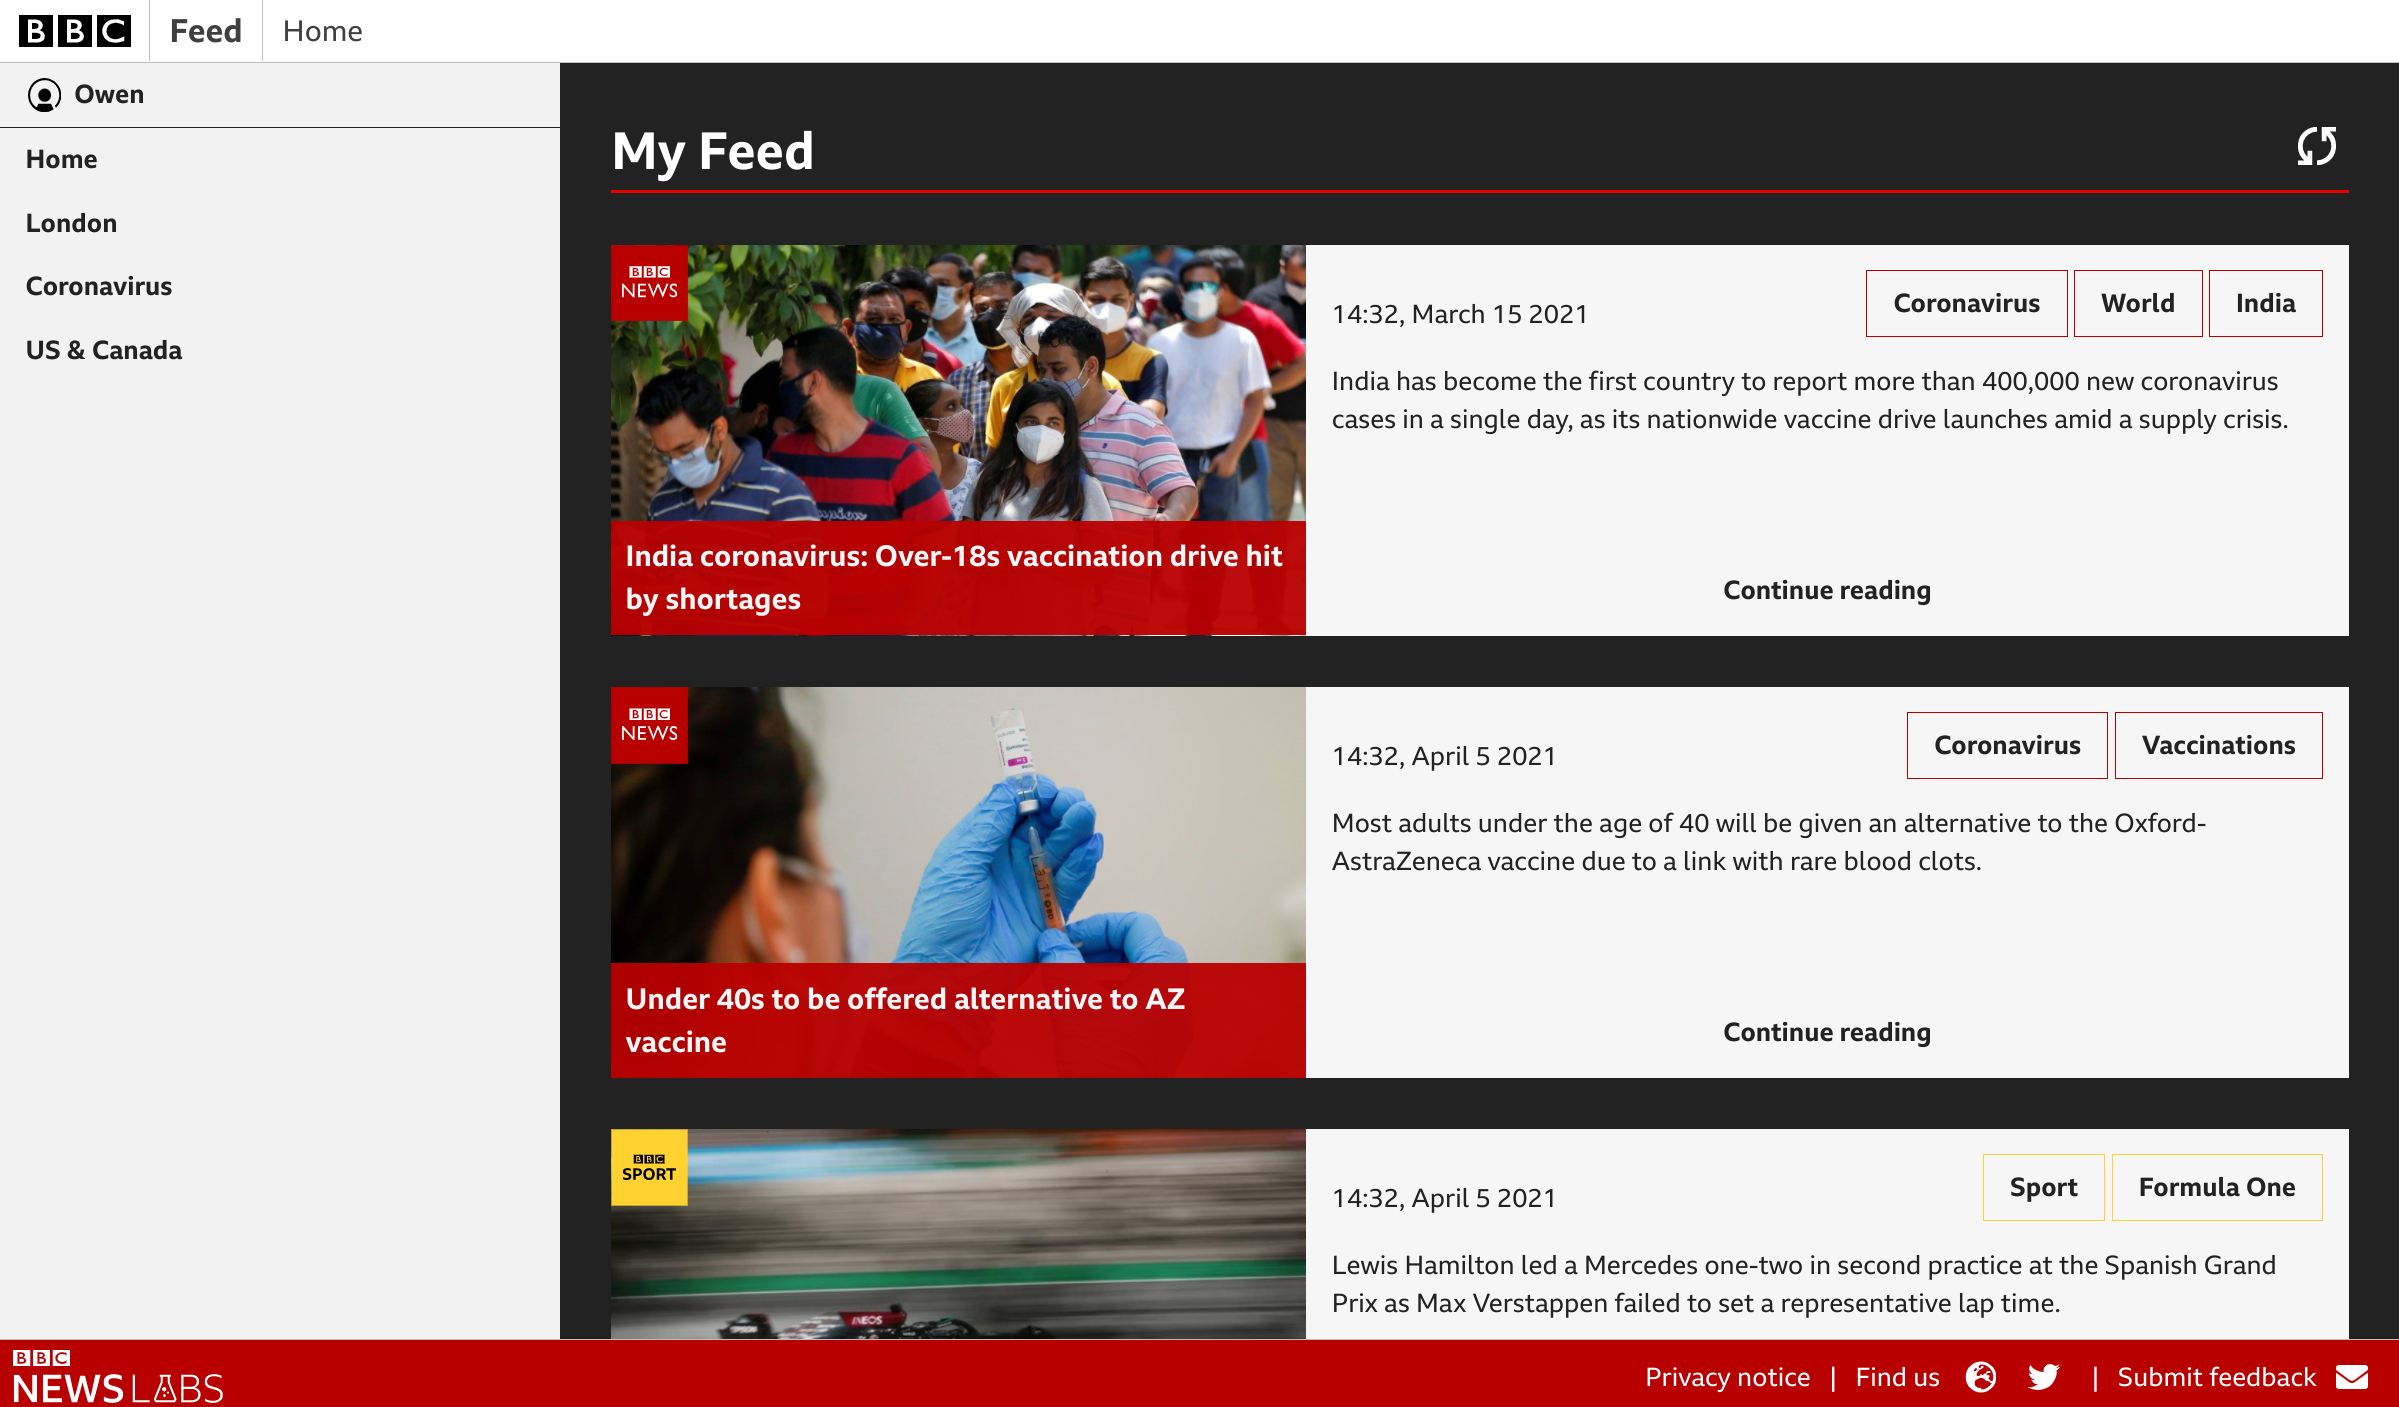
\includegraphics[width=.95\linewidth]{../img/sc-home-logged-in.png}}
      \end{minipage}\par\medskip

      \begin{minipage}{.5\linewidth}
        \centering
        \subfloat[Single Topic]{\label{fig:home3}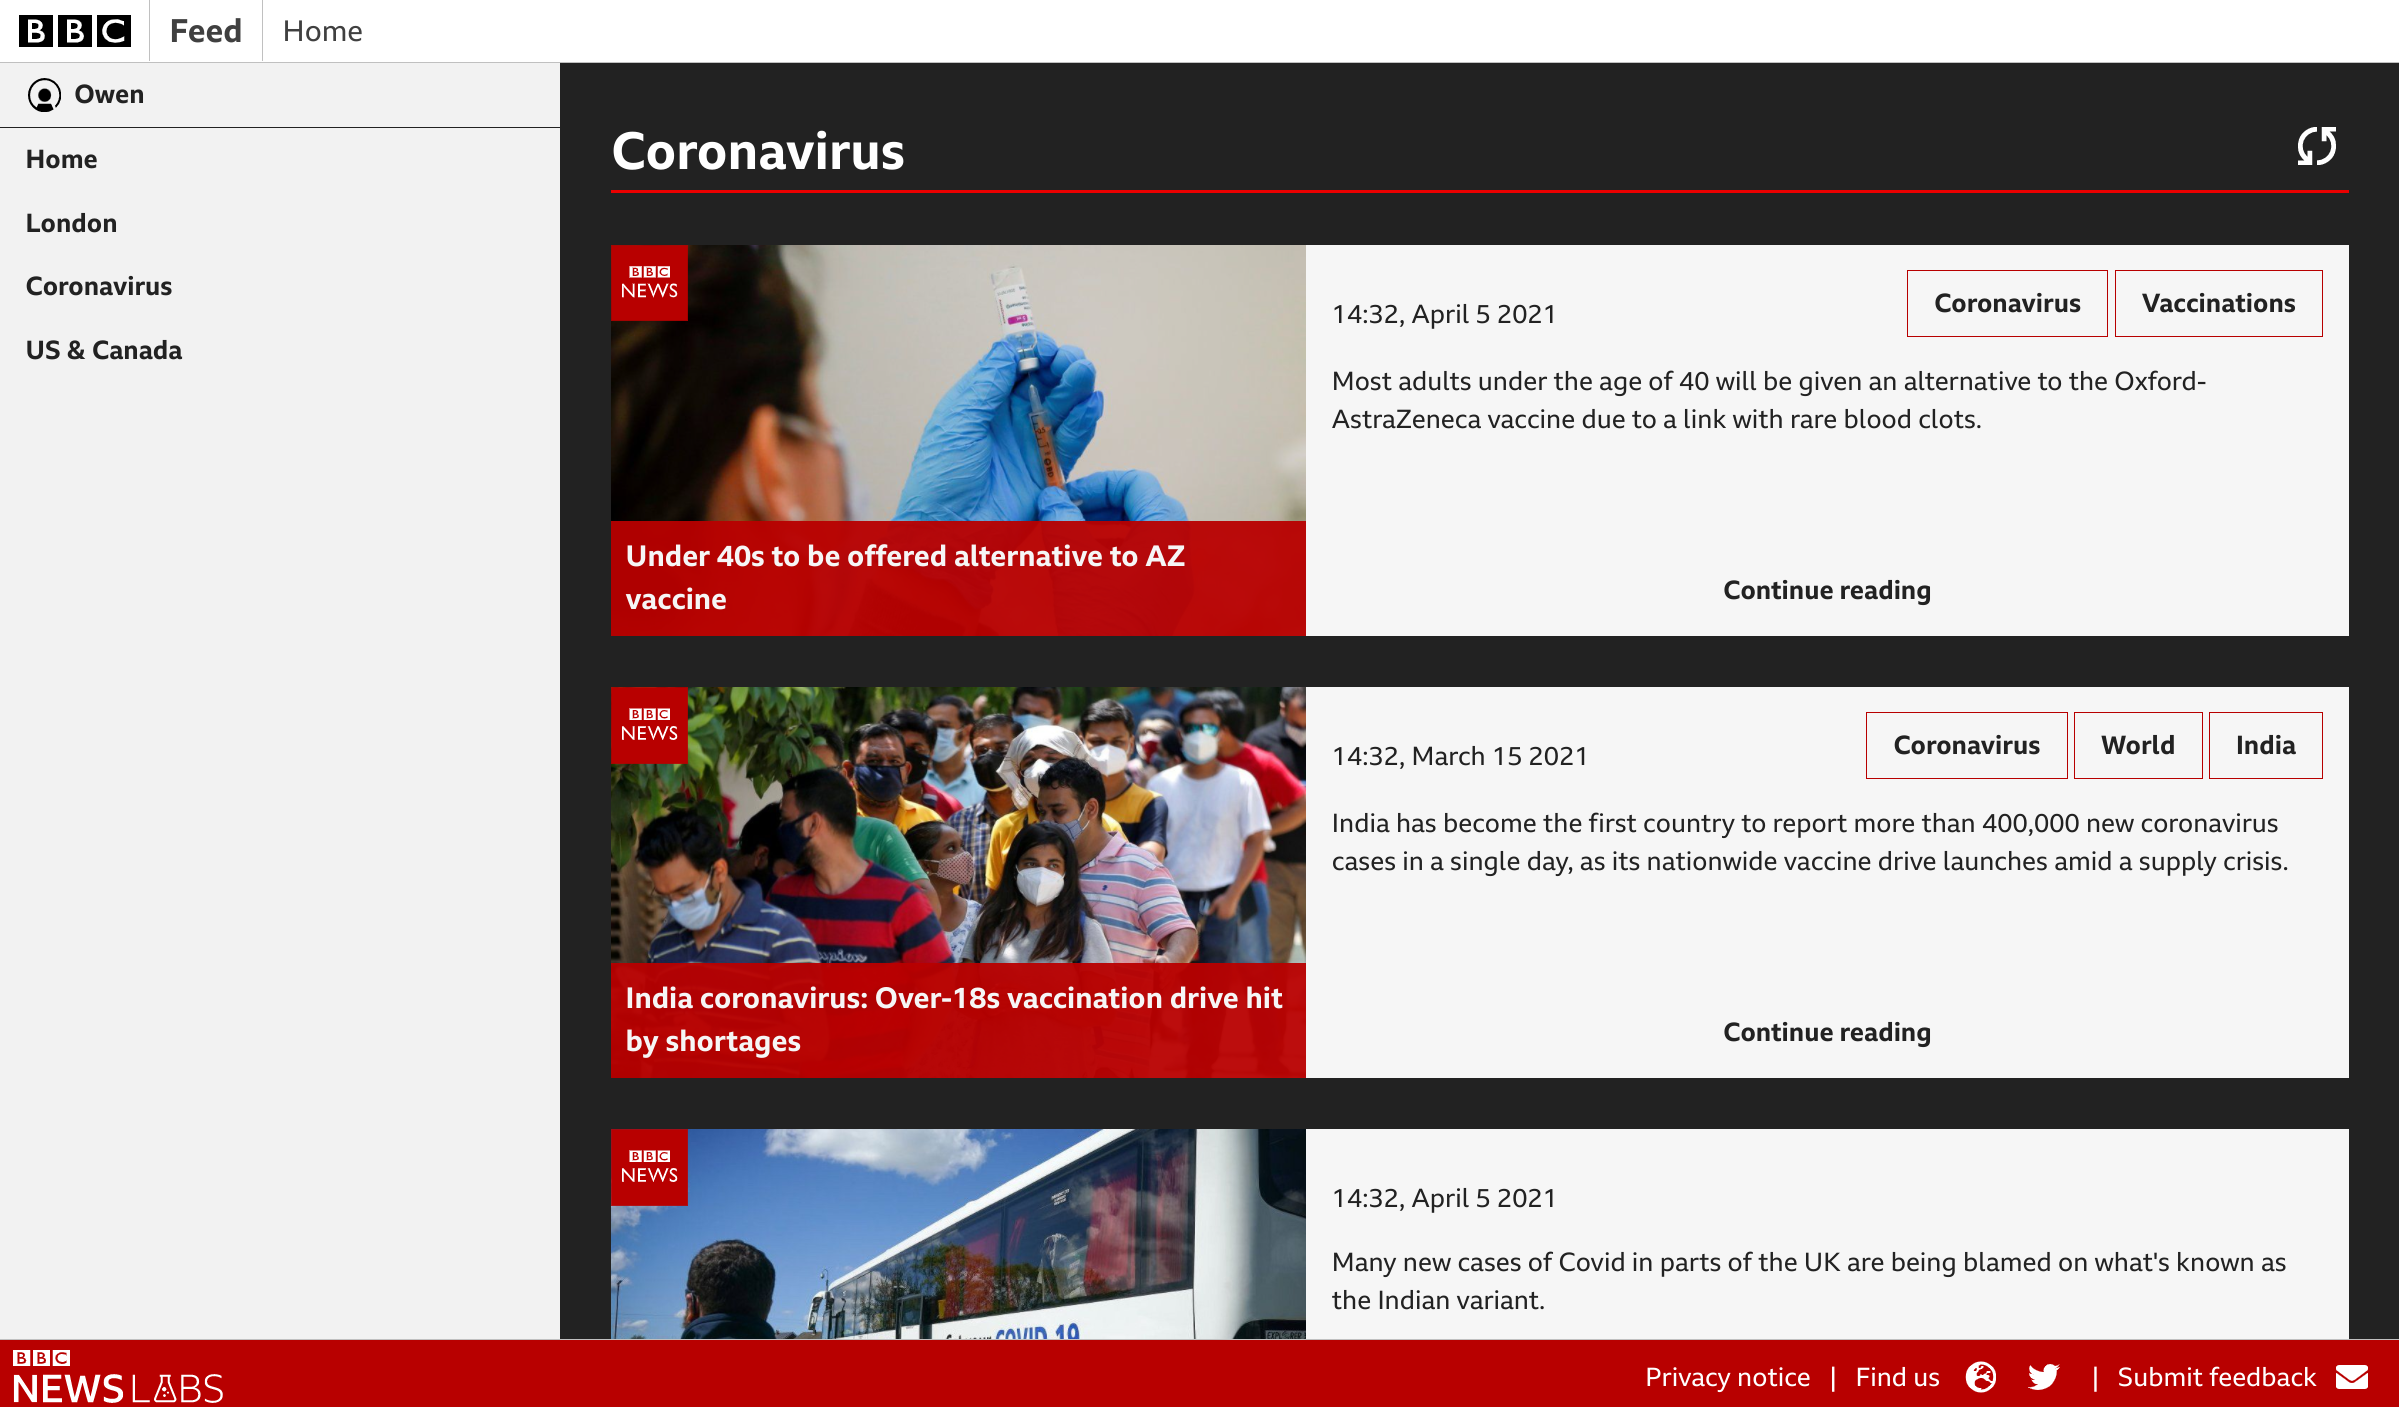
\includegraphics[width=.95\linewidth]{../img/sc-topic.png}}
      \end{minipage}%
      \begin{minipage}{.5\linewidth}
        \centering
        \subfloat[Single Story]{\label{fig:home4}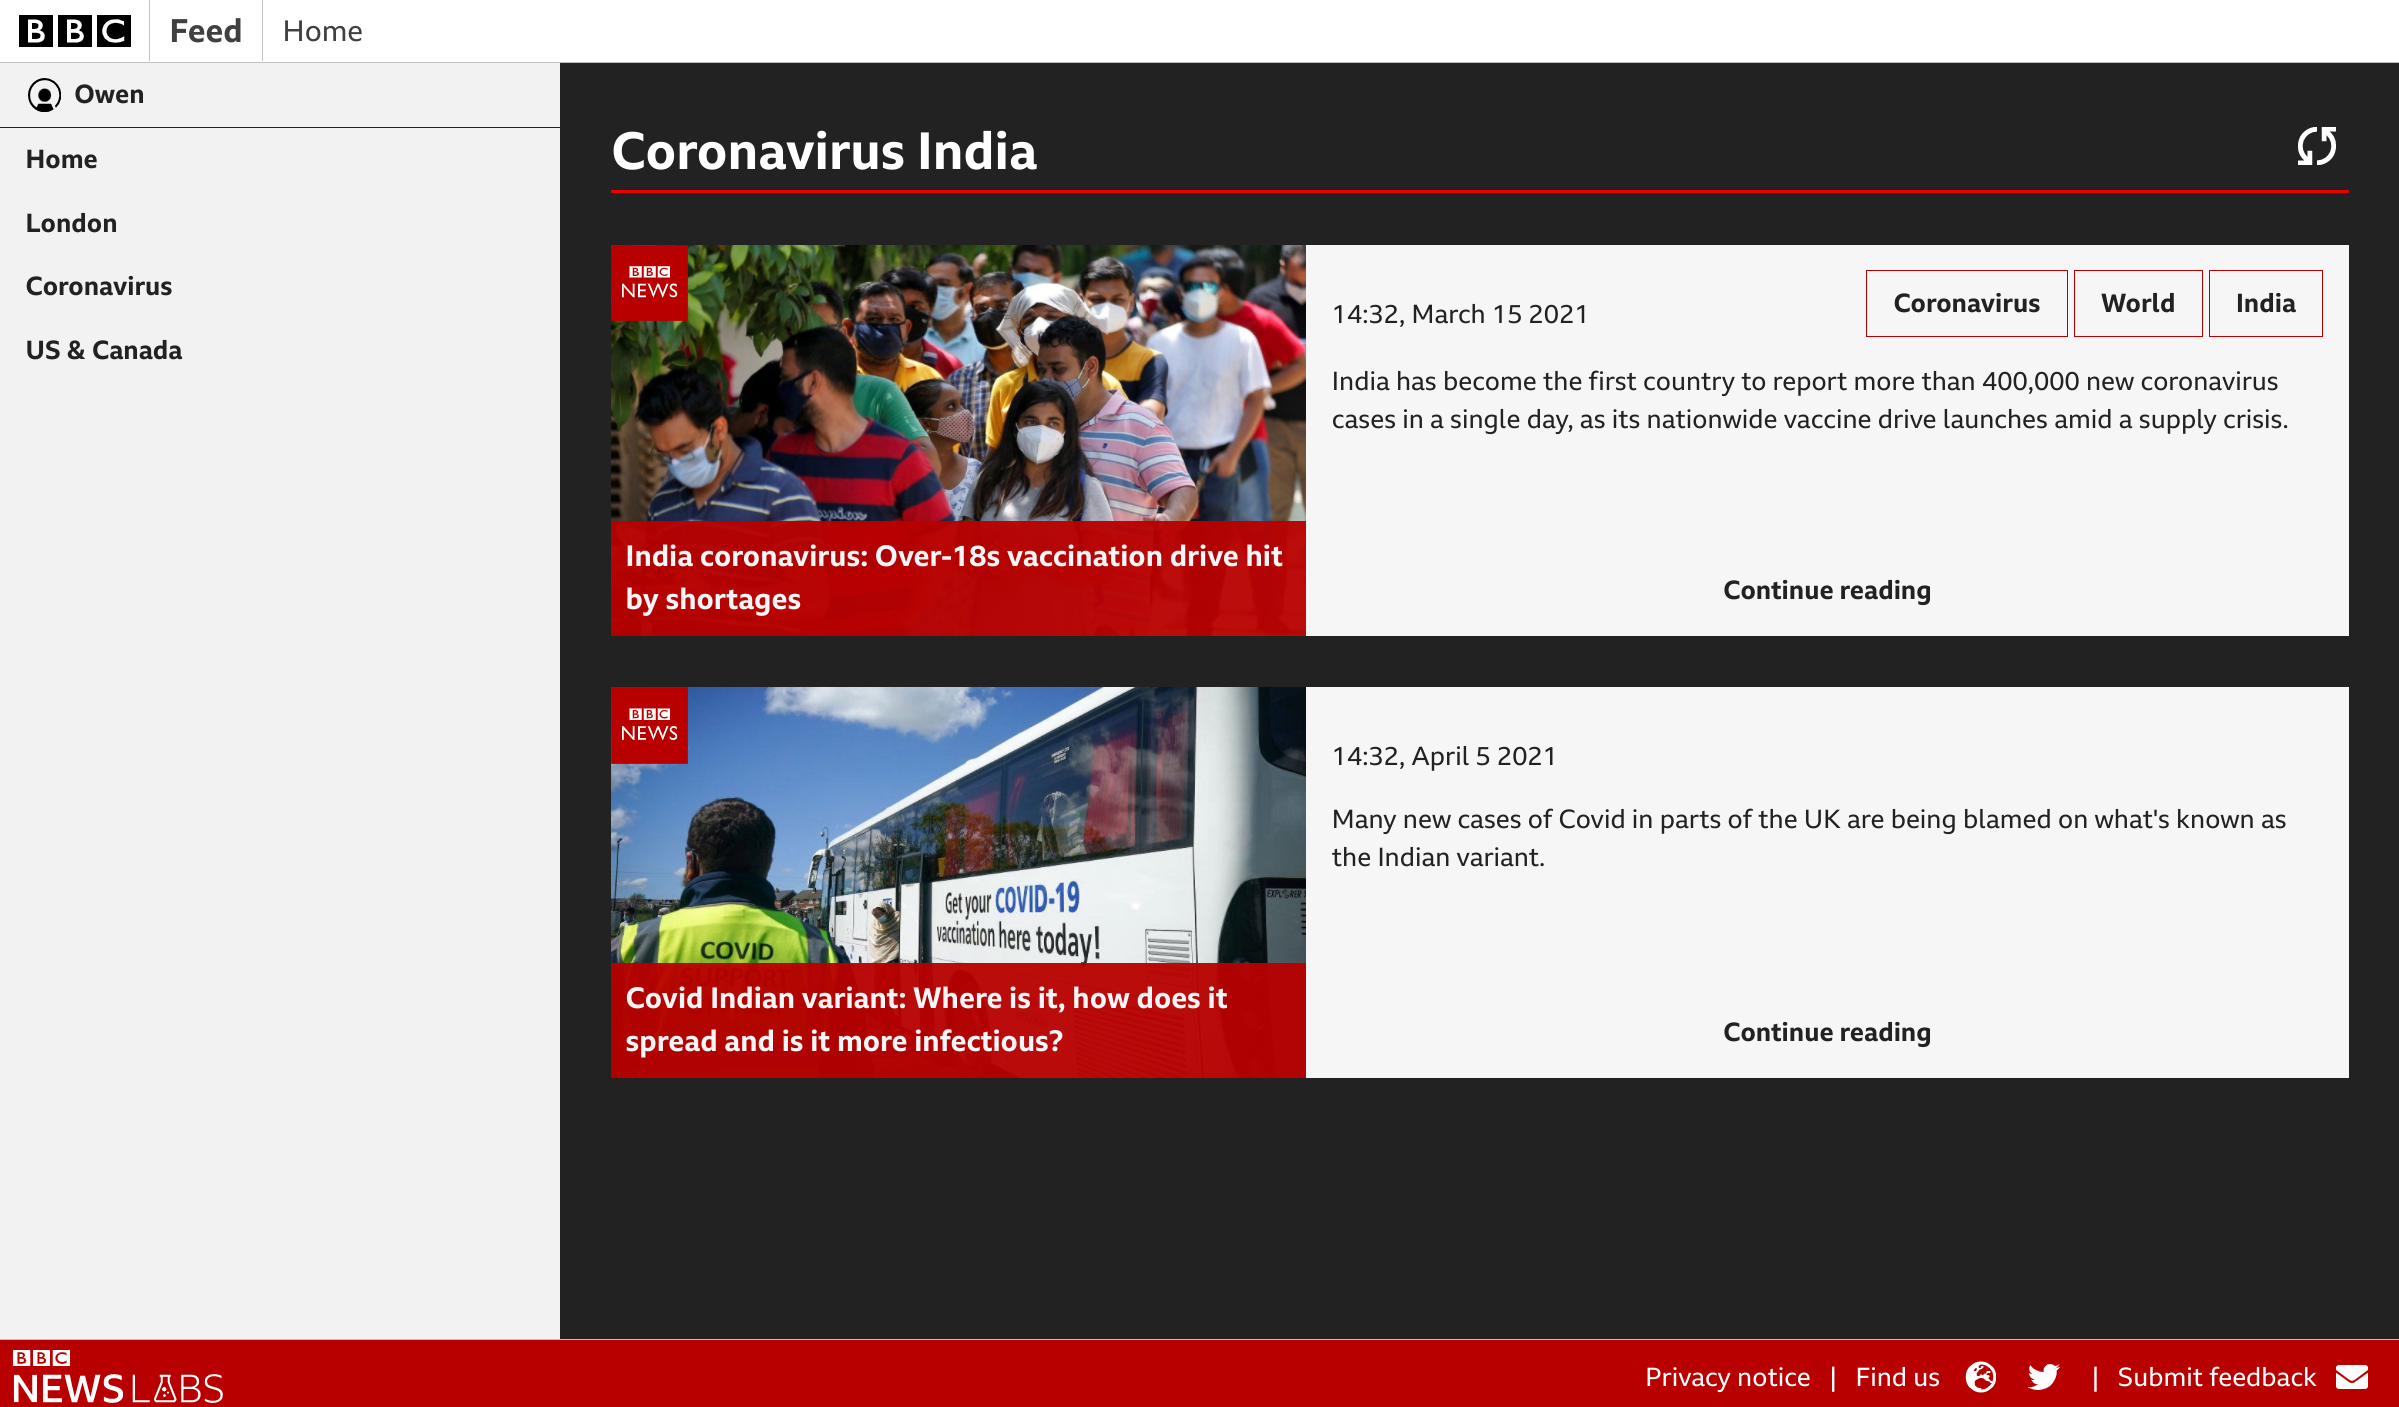
\includegraphics[width=.95\linewidth]{../img/sc-story.png}}
      \end{minipage}
      \centering
      \subfloat[Expanded post]{\label{fig:home5}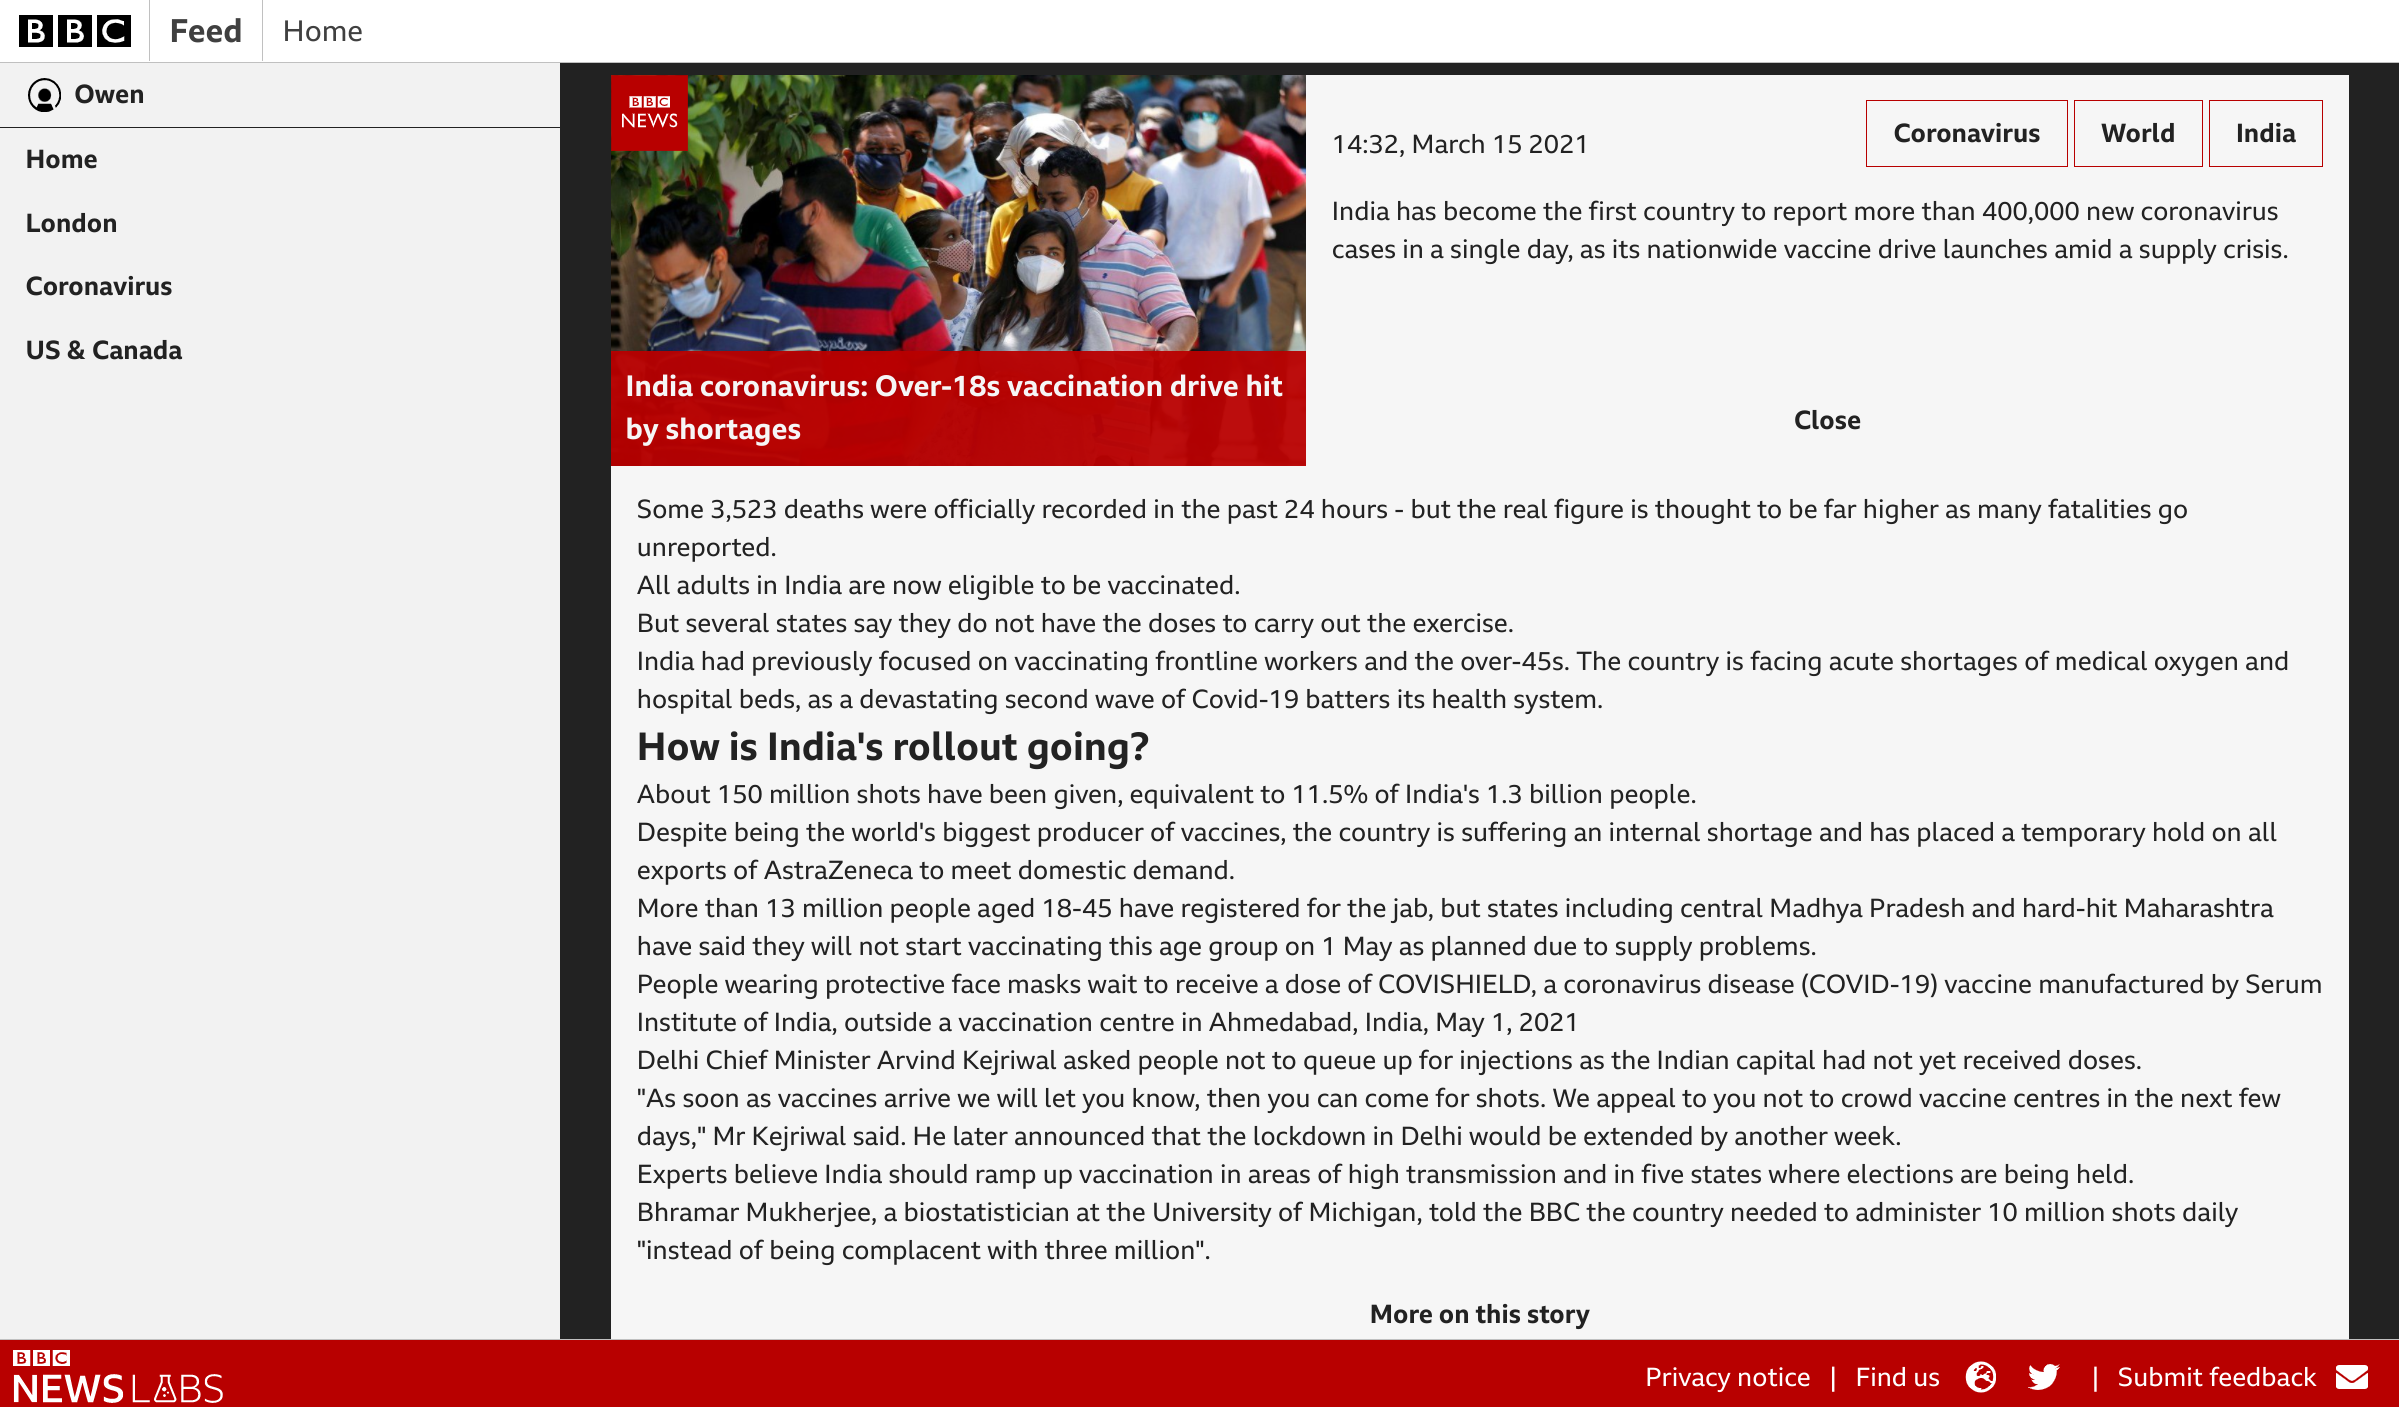
\includegraphics[width=.475\linewidth]{../img/sc-post.png}}

      \caption{The home page}
      \label{fig:home}
    \end{figure}

    The home page is split into three main sections: the header and footer, the
    navigation panel on the left and the feed content on the right. The header
    and footer were provided by BBC News Labs and have been used to show that
    this is a prototype application and not an actual BBC product. In a
    production version of this interface the footer would be removed entirely
    and the header would be replaced with a standard BBC header that would
    contain links to other BBC services.

    The navigation panel is designed to allow easy navigation to any of the
    topics a user might be interested in. It has two states: signed in and
    signed out. In the signed out state it shows a few buttons that link to
    popular topics, in the real system these would be decided using viewing
    trends but for this project they are pre-set. In the signed in state this
    area contains a list of buttons that link to the topics that the user has
    selected in their profile. In either state the buttons are themed according
    to the brand of their topic by using the brand colour as a background when
    the user hovers over them. Due to the various brand colours being used the
    text had to be inverted sometimes to ensure a high contrast for readability
    reasons.

    The feed content contains the list of current posts the user is consuming.
    This list is presented on a dark background in order to draw the users
    attention to the content and to provide separation between each post. At the
    top there is a heading that changes depending on the content being
    displayed. If the user is viewing a topic or story then the title of this is
    shown here, otherwise it defaults to displaying 'My Feed'. There is a
    refresh button alongside this heading however this is non functional in this
    project as new posts cannot be added to the system dynamically.

    Each post in the feed is also split into three sections: the post image,
    post summary and the post body. The body is hidden by default and requires
    the user click on 'Continue reading' in order to show it, this can be seen
    in fig. \ref{fig:home5}. The body of the post itself is deliberately left
    undefined as different types of post will want to use this area in unique
    ways. In the example data a few paragraphs and headings are used to show how
    a standard news article might appear. After this there is a button that
    allows the user to view more posts in the same story as the current post.
    This uses the brand of the post as a highlight colour as the user hovers
    over it to show that it is interactable.

    The post image uses an image that is relevant to the post as a background
    element, with the headline and brand logo drawn on top of the image. This
    use of branding on top of the image helps to tie the post to the brand and
    make each brand stand out from the others. This is the boldest use of the
    brand colours in the user interface and brings a lot of colour and interest
    to the otherwise very monotone interface.

    The post summary contains metadata about the post such as the date it was
    created, a brief summary of the content, and its associated tags (if any).
    This is followed by a 'Continue reading' button that darkens its background
    when hovered to show interactivity. This is different from the other
    buttons that use a bright colour when hovered, this was done to show that
    this button won't take the user to a new page, instead it will change the
    current page in some way. The posts tags are coloured according to their
    respective brands. The sizing of the borders and negative space in these
    elements was taken from the BBC News web site to ensure that this interface
    would look correct as part of the BBC product range.

    \subsection{Login, Register and Profile Pages}

    \begin{figure}
      \begin{minipage}{.5\linewidth}
        \centering
        \subfloat[Log in]{\label{fig:up3}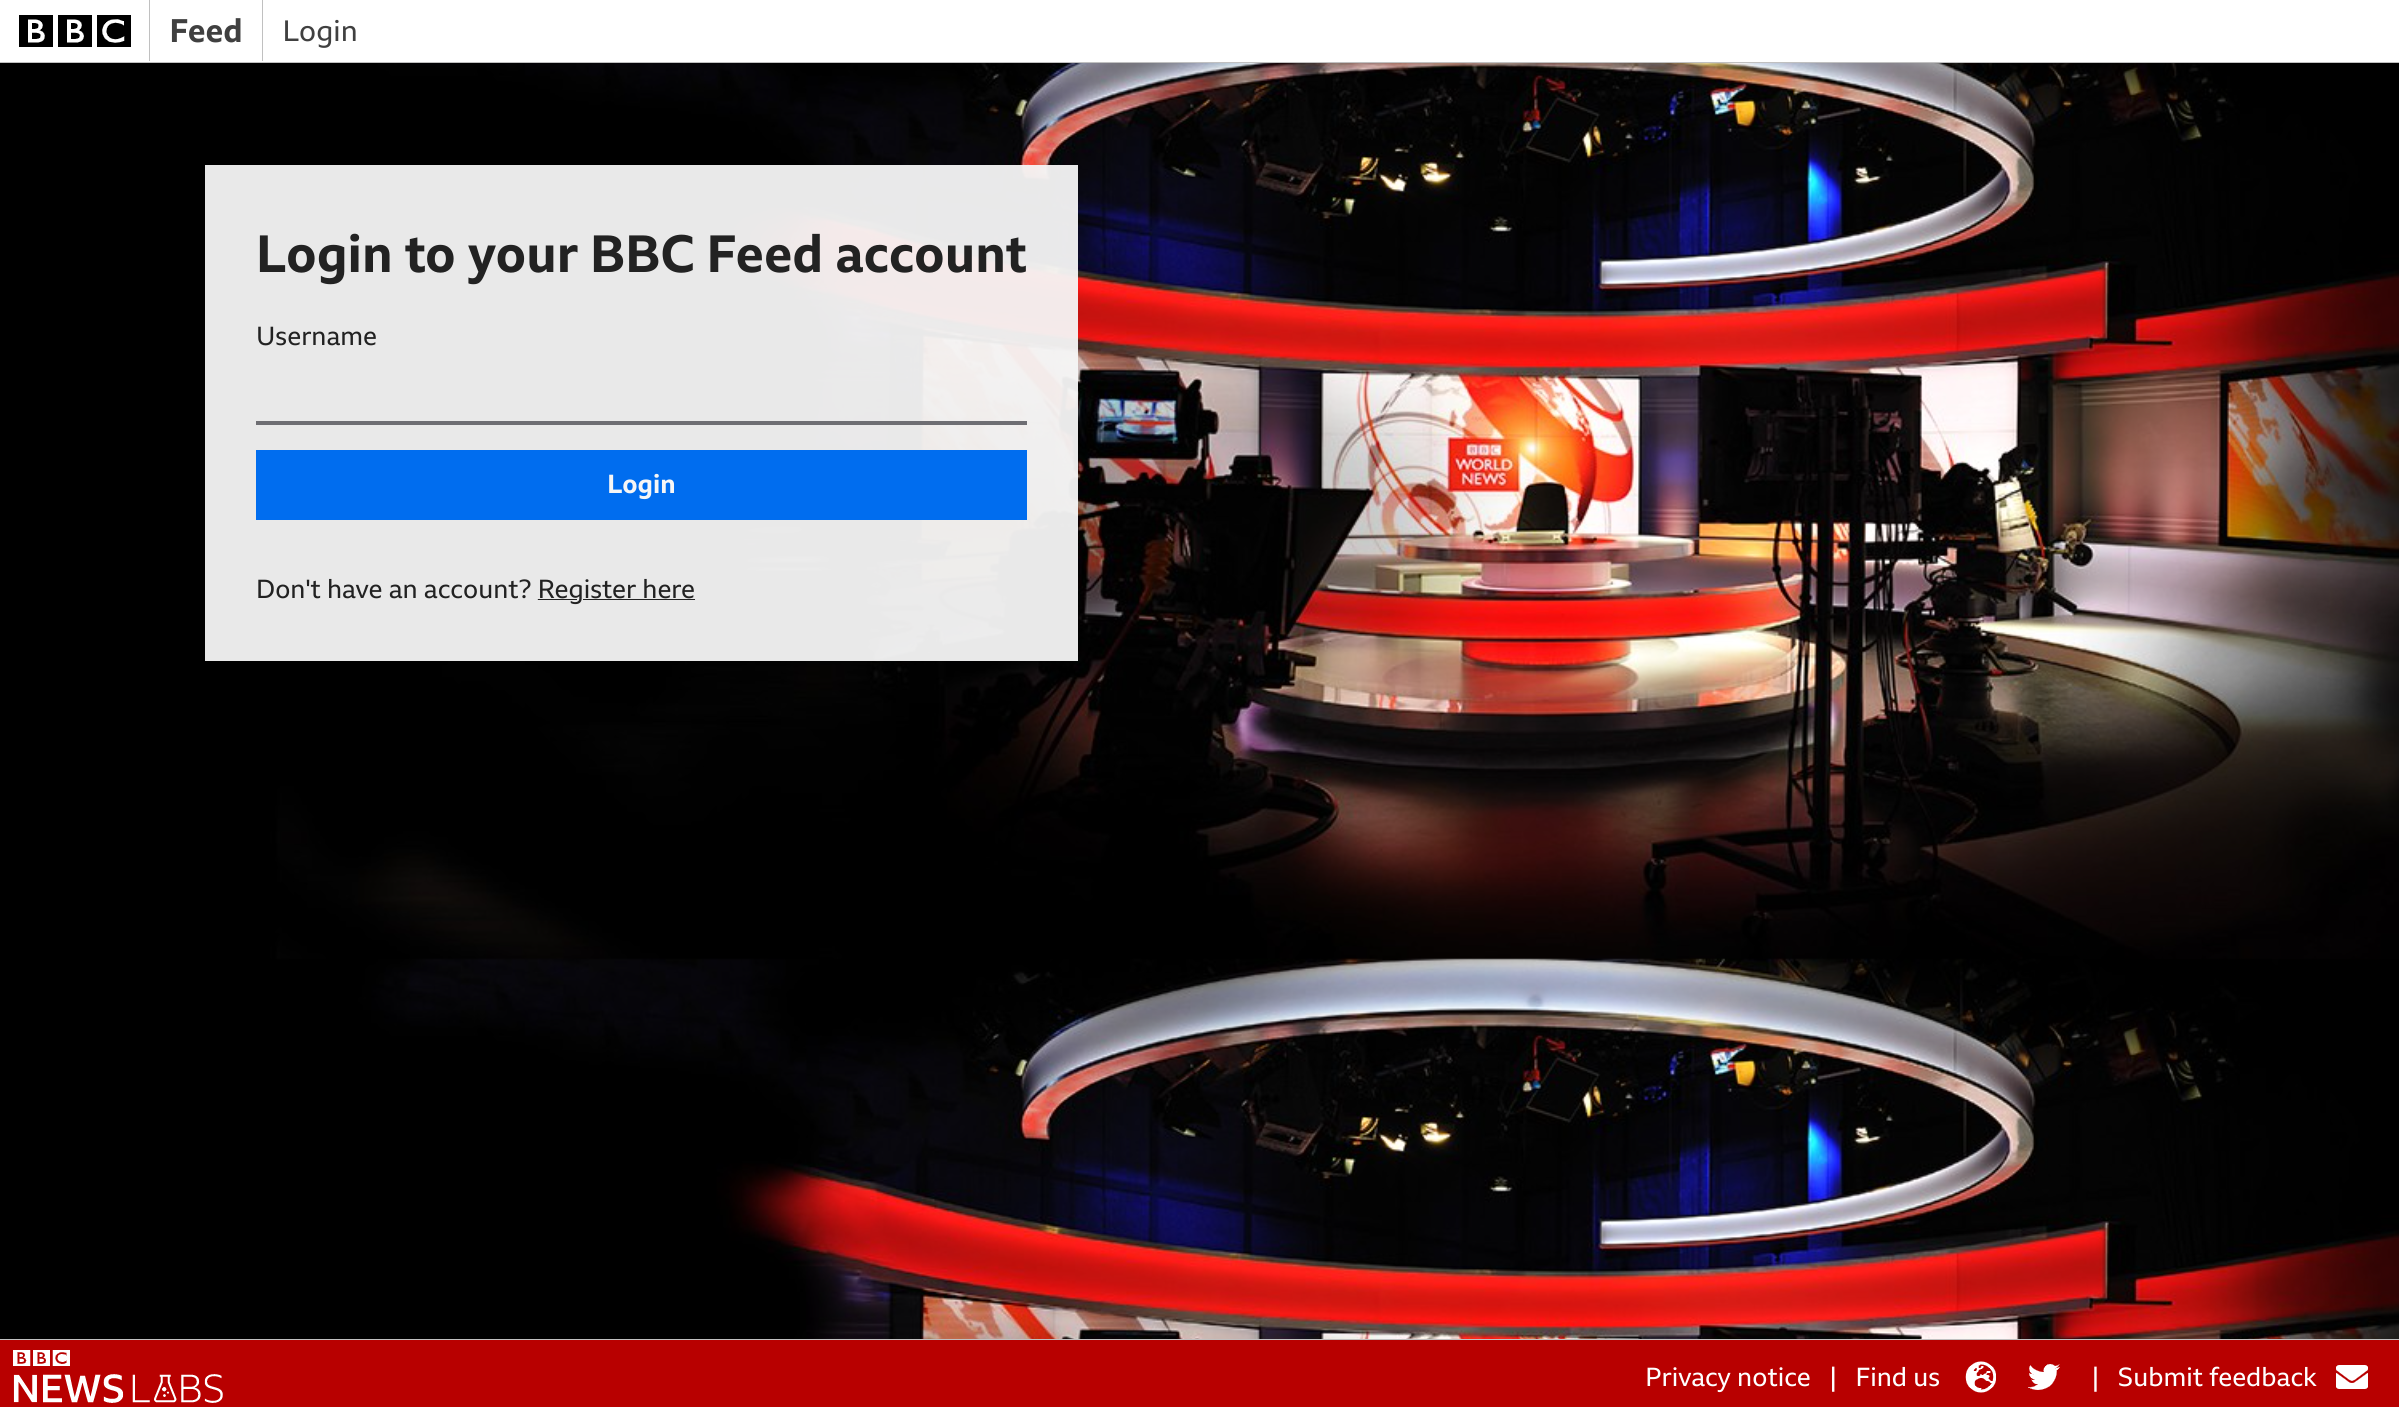
\includegraphics[width=.95\linewidth]{../img/sc-log-in.png}}
      \end{minipage}%
      \begin{minipage}{.5\linewidth}
        \centering
        \subfloat[Register]{\label{fig:up4}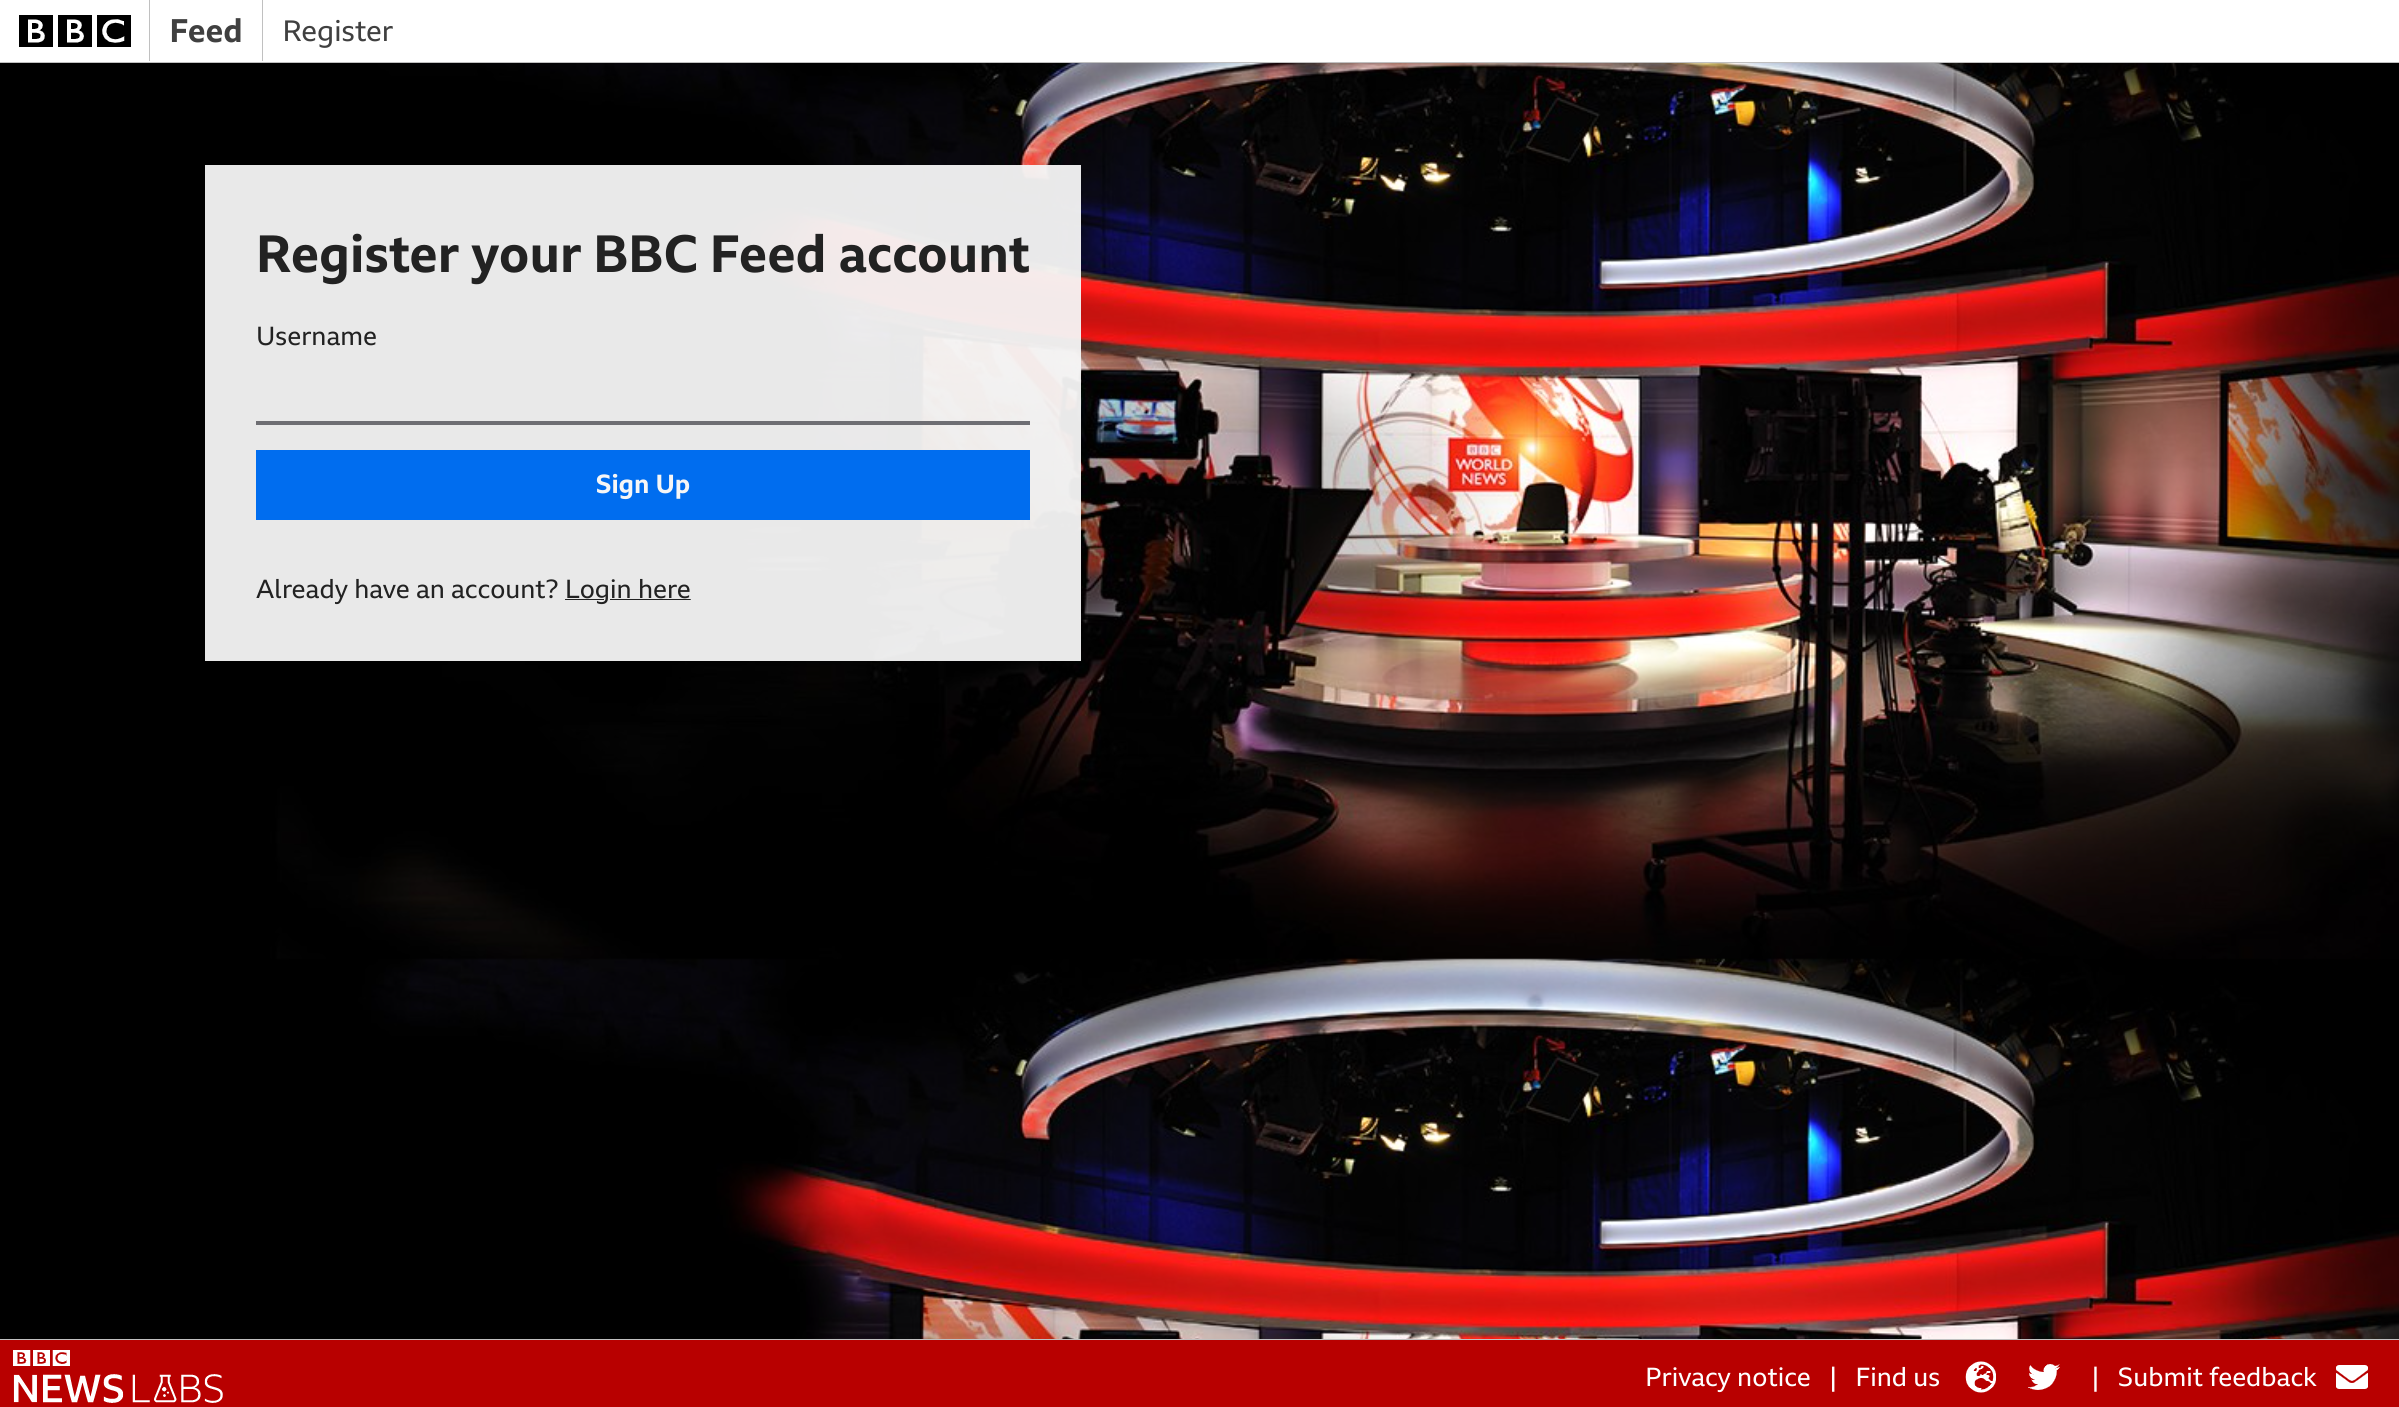
\includegraphics[width=.95\linewidth]{../img/sc-register.png}}
      \end{minipage}
      \centering
      \subfloat[Profile]{\label{fig:up5}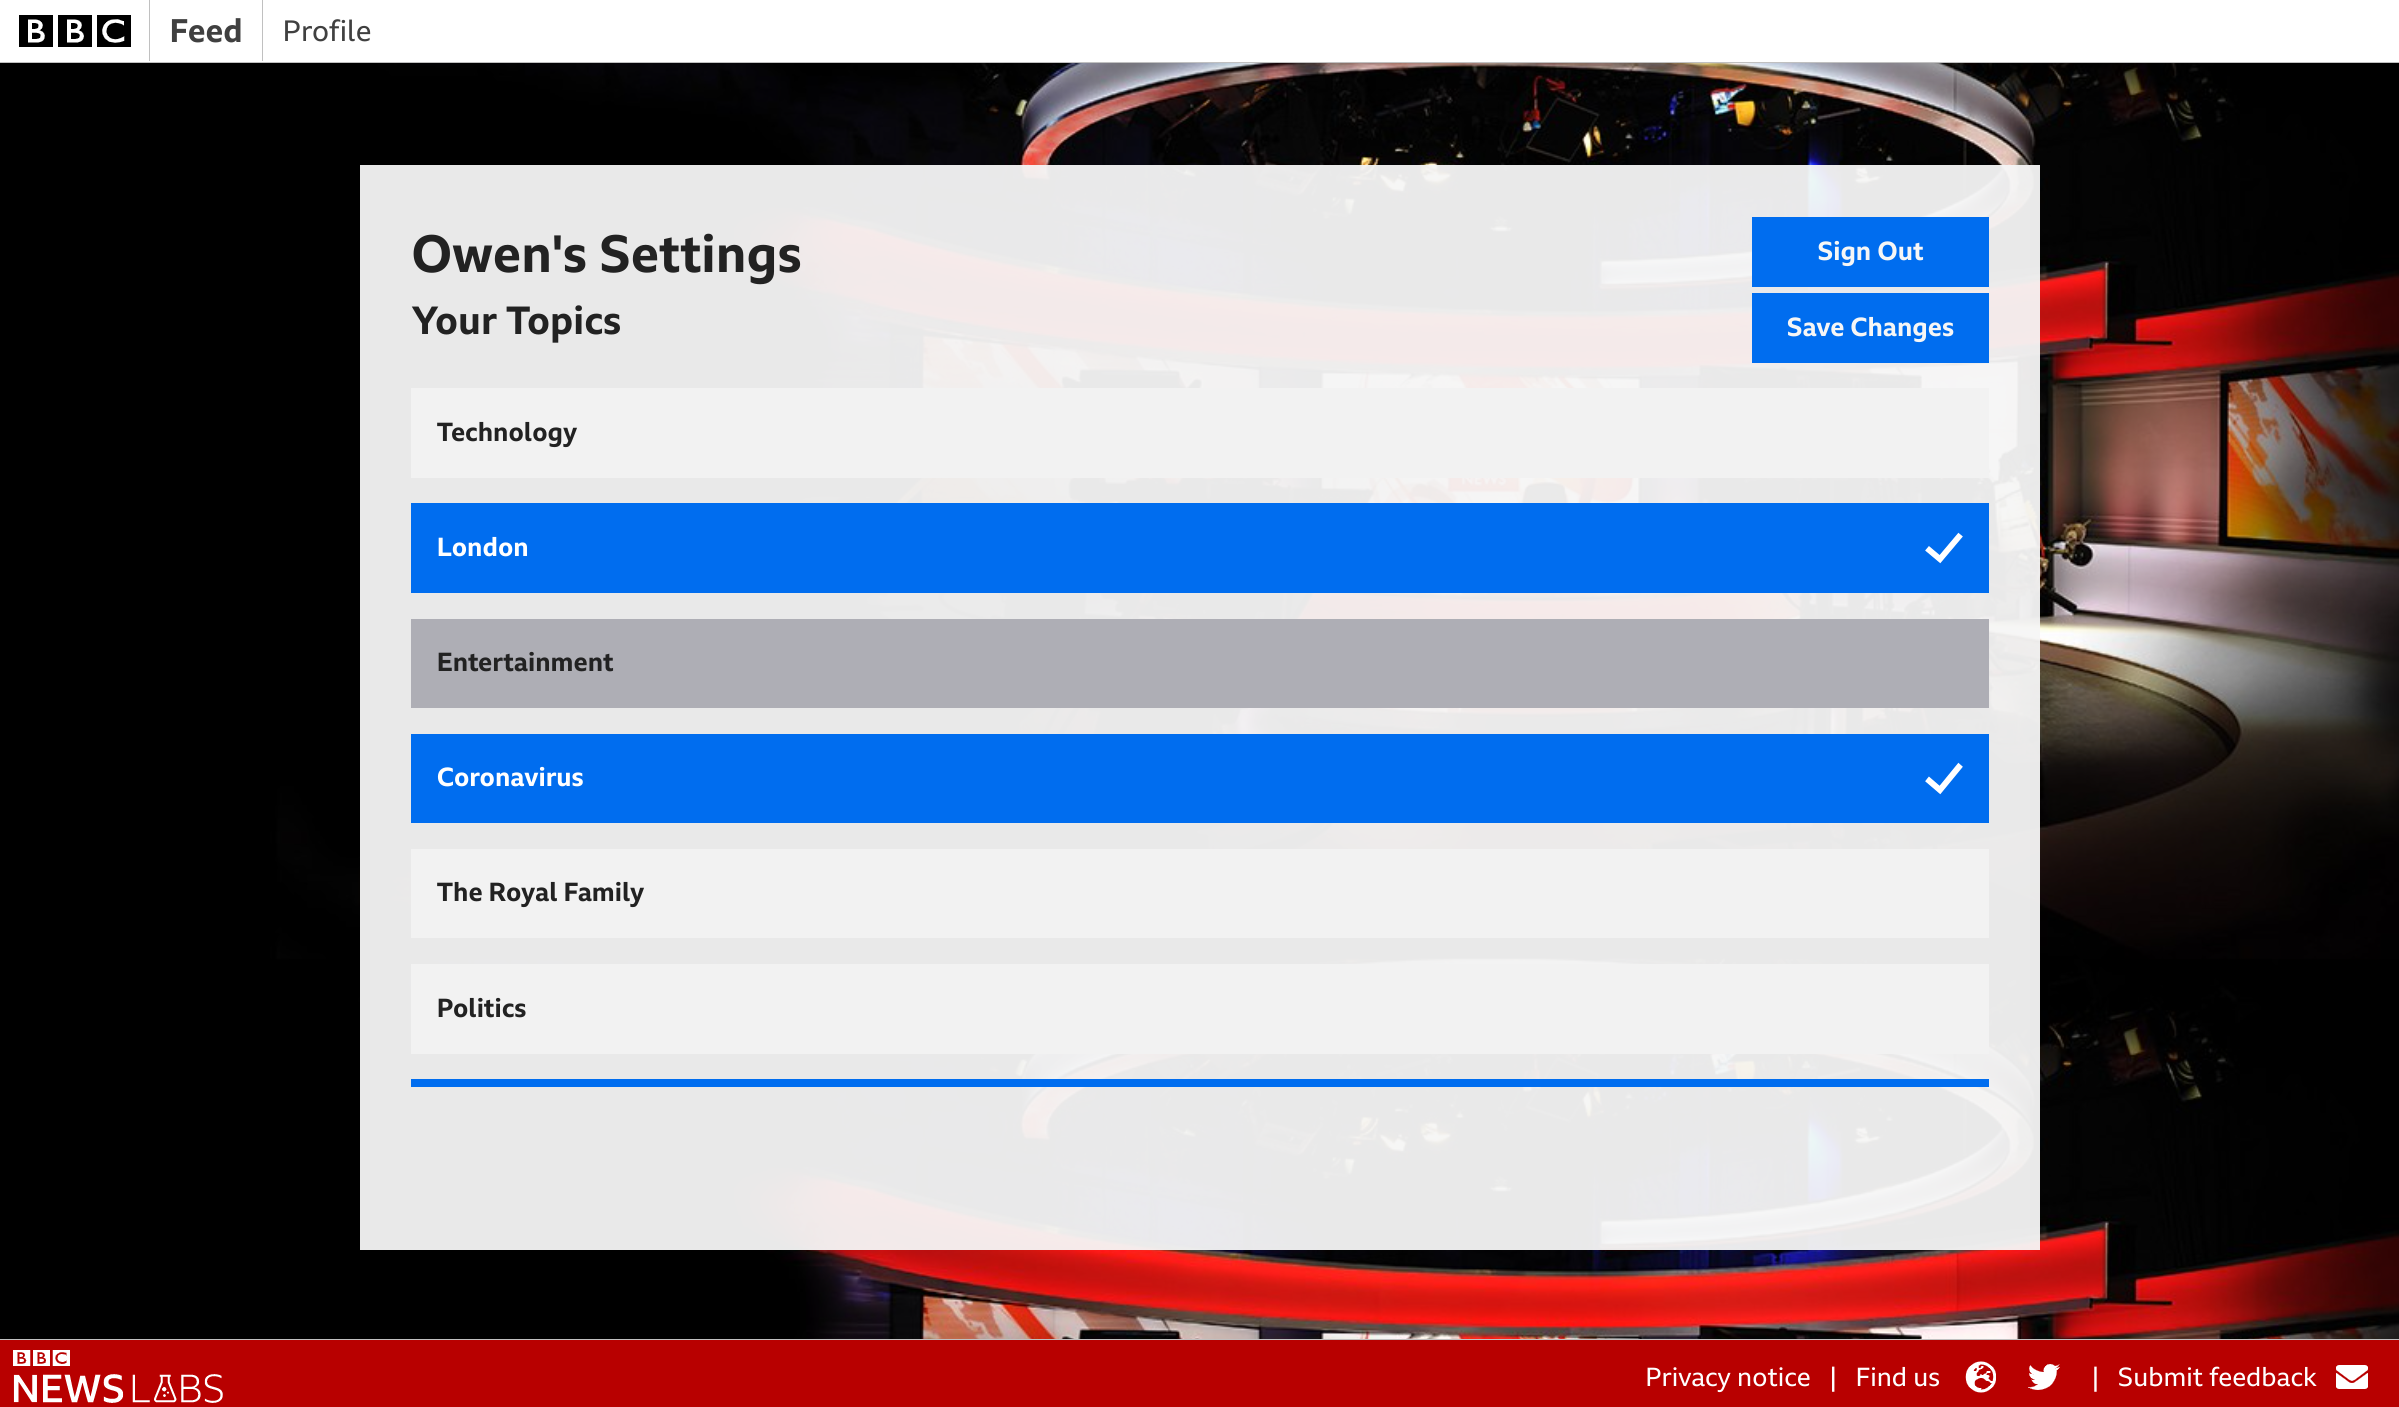
\includegraphics[width=.475\linewidth]{../img/sc-profile.png}}

      \caption{The user session pages}
      \label{fig:userpages}
    \end{figure}

    These three pages share a lot of stylistic elements between them. This was
    done to visually separate the content consumption pages from the user
    management pages. As these pages don't showcase any BBC content they
    couldn't use brand colours to highlight interface elements. Instead a bright
    blue was used, this was chosen from the official BBC colour palette, but it
    is not used for any BBC brands, allowing these elements to stand out from
    the rest of the interface.

    The use of an image in the background matches other BBC products that also
    employ this technique. This provides some interest to pages that would
    otherwise feel very utilitarian. The background was chosen to be dark to
    allow the user interface elements on top of it to stand out, this draws the
    users focus to the parts of the page they need to interact with. The
    specific image was chosen as it evokes a sense of being behind the scenes,
    this allows the user to feel like nothing is being hidden from them.
    Similar techniques are being used across the BBC to show audiences the
    sides of broadcasting that are normally hidden away.

    The profile page was not worked on extensively as in a production system
    this would be replaced with the BBC's centralised user sign in system. The
    blue colours have been used here to highlight interactable elements, but
    this page shows that this can be overbearing if used too heavily. An
    improvement to this page would be to make the buttons grey-scale and only
    show the blue colour when the user hovered over the elements.

\section{Informal Evaluation}

  Once the system was completed it was necessary to evaluate it in order to
  determine if the project was a success. A user study was considered, this would
  have involved allowing users to consume news through both the new system and
  existing news user interfaces and then collecting their feedback. This idea
  was rejected because of the limited data set available, it would not be
  possible for a user to consume news through the system in a realistic manner.
  This approach would also only test the user interface and would not evaluate
  the API aspect of the project.

  Due to these two issues it was instead decided to use an informal evaluation.
  A group of BBC News Labs developers, including the Head of Product, were
  selected and given a ten minute demonstration of the project. This showcased
  the user interface and API, while at the same time they were told about how
  the data was structured behind the scenes. After this they were free to ask
  questions about the project to ensure they understood the system as well as
  possible. Once they were satisfied with this they were asked to give their
  thoughts about the system, highlighting any positives or negatives that they
  could see along with their general thoughts about the project.

  The main negative they found was the user topic selection menu in the user
  profile page. They felt that this interface was 'clunky' and that many users
  would not be aware of it. Once they were told that this page replaced the user
  feedback buttons ('like'/'dislike') they agreed that this would solve the
  issues they had with the topic selection.

  Another issue they found was the lack of any navigation elements when on the
  login, register and profile pages. They felt that could leave users feeling
  stranded. The browsers built in back button fulfils this role, however a home
  button should have been added to these pages and this was an oversight when
  developing the user interface.

  All the developers agreed that the interface was well designed in general,
  with clear synergy to existing BBC platforms which they said shows how this
  project could be integrated into a wider system. The use of spot colours to
  both draw the users focus and identify branding was highlighted as a good
  design element. They liked the consistent use of negative space to break up
  the pages and keep them readable whilst still conveying dense information.
  They thought that the infinite scrolling idea was an interesting development
  on the traditional news user interface and they thought that a full user study
  in this field would be worthwhile.

  The API was of specific interest to some of the developers. They felt that if
  this project was polished and deployed then it would offer easy access to a
  rich collection of structured data that could enable many other projects that
  are currently not possible. They also liked the concept of many different
  sources feeding into this single system, although they did highlight that
  engineering a system to process this data at a large scale would be a
  significant challenge.

  The connected nature of the data excited some of the developers. They liked
  the idea of a Python library that they could import into their own projects to
  get easy access to this data without having to worry about making API calls
  themselves. They mentioned that it would be good to port this library to other
  languages that the BBC uses regularly such as NodeJS, Java and C++.

  Overall the developers had a positive response to the project, and they said
  that it is something News Labs would consider developing further in the
  future. They mentioned that it would be challenging for their team to take on
  however due to the need for long term maintenance which, as an innovation
  focused team, they don't provide. If a suitable team was found that could take
  on the task of deploying and maintaining this system however they believe it
  would be worth investing development time into furthering this idea.

\section{Discussion}

  This project has highlighted the impact that changing a user interface can
  have on a news consumption platform. By focusing the user interface and data
  structure around the ways in which the content is interconnected, a functional
  and eye catching user interface has been built. The full impact of such an
  interface will need to be studied further in order to evaluate the effect this
  has on the user experience and user retention. However from this work alone it
  is clear that there are many interface aspects that can be taken from other
  platforms where they have shown success, and adapted to deliver news content.
  This raises questions about what other models could be adapted in the same
  way, either again from social media or from the wider internet.

  The feedback from the developers shows that a clean user interface with a
  singular goal can be both easy to use and pleasing to look at. It may be that
  this benefit becomes lessened or removed entirely if it was integrated into a
  production environment. This would require adding many interface elements in
  order to integrate the application with the rest of the BBC product range
  which may harm the focused nature of the user interface.

  The data interface however holds more interest for future research, the
  benefits this provides are twofold. Firstly having a service that can accept
  data on nearly any part of a news story and link these to other relevant parts
  would be invaluable to any large media organisation. Secondly having this
  central service that could be queried at will would allow various projects and
  research to analyse the news content in near real time. Being able to traverse
  the data in order to find other connected data would enable many currently
  disparate systems to become interconnected. Implementing this would not be
  easy however as it would require many monolithic systems to be modified or
  replaced which would cost large sums of money and time, however it may well be
  worth the effort in the long run.

\section{Conclusion}

%To-Do: Write conclusion

\section{Recommendations}

%To-Do: Write Recomendations

\bibliography{final_report}

\end{document}
